% Options for packages loaded elsewhere
\PassOptionsToPackage{unicode}{hyperref}
\PassOptionsToPackage{hyphens}{url}
%
\documentclass[
]{article}
\usepackage{lmodern}
\usepackage{amssymb,amsmath}
\usepackage{ifxetex,ifluatex}
\ifnum 0\ifxetex 1\fi\ifluatex 1\fi=0 % if pdftex
  \usepackage[T1]{fontenc}
  \usepackage[utf8]{inputenc}
  \usepackage{textcomp} % provide euro and other symbols
\else % if luatex or xetex
  \usepackage{unicode-math}
  \defaultfontfeatures{Scale=MatchLowercase}
  \defaultfontfeatures[\rmfamily]{Ligatures=TeX,Scale=1}
\fi
% Use upquote if available, for straight quotes in verbatim environments
\IfFileExists{upquote.sty}{\usepackage{upquote}}{}
\IfFileExists{microtype.sty}{% use microtype if available
  \usepackage[]{microtype}
  \UseMicrotypeSet[protrusion]{basicmath} % disable protrusion for tt fonts
}{}
\makeatletter
\@ifundefined{KOMAClassName}{% if non-KOMA class
  \IfFileExists{parskip.sty}{%
    \usepackage{parskip}
  }{% else
    \setlength{\parindent}{0pt}
    \setlength{\parskip}{6pt plus 2pt minus 1pt}}
}{% if KOMA class
  \KOMAoptions{parskip=half}}
\makeatother
\usepackage{xcolor}
\IfFileExists{xurl.sty}{\usepackage{xurl}}{} % add URL line breaks if available
\IfFileExists{bookmark.sty}{\usepackage{bookmark}}{\usepackage{hyperref}}
\hypersetup{
  pdftitle={Machine Learning Algorithms Documentation},
  pdfauthor={Geiser, Gruen, Hefti, Kuster},
  hidelinks,
  pdfcreator={LaTeX via pandoc}}
\urlstyle{same} % disable monospaced font for URLs
\usepackage[margin=1in]{geometry}
\usepackage{color}
\usepackage{fancyvrb}
\newcommand{\VerbBar}{|}
\newcommand{\VERB}{\Verb[commandchars=\\\{\}]}
\DefineVerbatimEnvironment{Highlighting}{Verbatim}{commandchars=\\\{\}}
% Add ',fontsize=\small' for more characters per line
\usepackage{framed}
\definecolor{shadecolor}{RGB}{248,248,248}
\newenvironment{Shaded}{\begin{snugshade}}{\end{snugshade}}
\newcommand{\AlertTok}[1]{\textcolor[rgb]{0.94,0.16,0.16}{#1}}
\newcommand{\AnnotationTok}[1]{\textcolor[rgb]{0.56,0.35,0.01}{\textbf{\textit{#1}}}}
\newcommand{\AttributeTok}[1]{\textcolor[rgb]{0.77,0.63,0.00}{#1}}
\newcommand{\BaseNTok}[1]{\textcolor[rgb]{0.00,0.00,0.81}{#1}}
\newcommand{\BuiltInTok}[1]{#1}
\newcommand{\CharTok}[1]{\textcolor[rgb]{0.31,0.60,0.02}{#1}}
\newcommand{\CommentTok}[1]{\textcolor[rgb]{0.56,0.35,0.01}{\textit{#1}}}
\newcommand{\CommentVarTok}[1]{\textcolor[rgb]{0.56,0.35,0.01}{\textbf{\textit{#1}}}}
\newcommand{\ConstantTok}[1]{\textcolor[rgb]{0.00,0.00,0.00}{#1}}
\newcommand{\ControlFlowTok}[1]{\textcolor[rgb]{0.13,0.29,0.53}{\textbf{#1}}}
\newcommand{\DataTypeTok}[1]{\textcolor[rgb]{0.13,0.29,0.53}{#1}}
\newcommand{\DecValTok}[1]{\textcolor[rgb]{0.00,0.00,0.81}{#1}}
\newcommand{\DocumentationTok}[1]{\textcolor[rgb]{0.56,0.35,0.01}{\textbf{\textit{#1}}}}
\newcommand{\ErrorTok}[1]{\textcolor[rgb]{0.64,0.00,0.00}{\textbf{#1}}}
\newcommand{\ExtensionTok}[1]{#1}
\newcommand{\FloatTok}[1]{\textcolor[rgb]{0.00,0.00,0.81}{#1}}
\newcommand{\FunctionTok}[1]{\textcolor[rgb]{0.00,0.00,0.00}{#1}}
\newcommand{\ImportTok}[1]{#1}
\newcommand{\InformationTok}[1]{\textcolor[rgb]{0.56,0.35,0.01}{\textbf{\textit{#1}}}}
\newcommand{\KeywordTok}[1]{\textcolor[rgb]{0.13,0.29,0.53}{\textbf{#1}}}
\newcommand{\NormalTok}[1]{#1}
\newcommand{\OperatorTok}[1]{\textcolor[rgb]{0.81,0.36,0.00}{\textbf{#1}}}
\newcommand{\OtherTok}[1]{\textcolor[rgb]{0.56,0.35,0.01}{#1}}
\newcommand{\PreprocessorTok}[1]{\textcolor[rgb]{0.56,0.35,0.01}{\textit{#1}}}
\newcommand{\RegionMarkerTok}[1]{#1}
\newcommand{\SpecialCharTok}[1]{\textcolor[rgb]{0.00,0.00,0.00}{#1}}
\newcommand{\SpecialStringTok}[1]{\textcolor[rgb]{0.31,0.60,0.02}{#1}}
\newcommand{\StringTok}[1]{\textcolor[rgb]{0.31,0.60,0.02}{#1}}
\newcommand{\VariableTok}[1]{\textcolor[rgb]{0.00,0.00,0.00}{#1}}
\newcommand{\VerbatimStringTok}[1]{\textcolor[rgb]{0.31,0.60,0.02}{#1}}
\newcommand{\WarningTok}[1]{\textcolor[rgb]{0.56,0.35,0.01}{\textbf{\textit{#1}}}}
\usepackage{graphicx,grffile}
\makeatletter
\def\maxwidth{\ifdim\Gin@nat@width>\linewidth\linewidth\else\Gin@nat@width\fi}
\def\maxheight{\ifdim\Gin@nat@height>\textheight\textheight\else\Gin@nat@height\fi}
\makeatother
% Scale images if necessary, so that they will not overflow the page
% margins by default, and it is still possible to overwrite the defaults
% using explicit options in \includegraphics[width, height, ...]{}
\setkeys{Gin}{width=\maxwidth,height=\maxheight,keepaspectratio}
% Set default figure placement to htbp
\makeatletter
\def\fps@figure{htbp}
\makeatother
\setlength{\emergencystretch}{3em} % prevent overfull lines
\providecommand{\tightlist}{%
  \setlength{\itemsep}{0pt}\setlength{\parskip}{0pt}}
\setcounter{secnumdepth}{-\maxdimen} % remove section numbering

\title{Machine Learning Algorithms Documentation}
\author{Geiser, Gruen, Hefti, Kuster}
\date{08/01/2021}

\begin{document}
\maketitle

{
\setcounter{tocdepth}{2}
\tableofcontents
}
\textbf{Data preparation}

\textbf{Dataset - German Housing Data}

Origin data set cleaned:

Variable rooms, bathrooms, bedrooms, floors, garages, Year\_built,
Year\_renovated changed from decimal to integer Subset with buildings up
to 20 rooms for our analysis created Rooms with .5 rounded up Levels of
the variable Energy\_source and Garagetype transformed.

\textbf{Load of the cleaned dataset} Read in the data \& have a short
glance with the head() function to get an idea of the dataset

\begin{Shaded}
\begin{Highlighting}[]
\NormalTok{data <-}\StringTok{ }\KeywordTok{read.csv}\NormalTok{(}\StringTok{'german_housing_cleaned.csv'}\NormalTok{,}\DataTypeTok{header =}\NormalTok{T, }\DataTypeTok{encoding=}\StringTok{'UTF-8'}\NormalTok{)}
\end{Highlighting}
\end{Shaded}

\textbf{Inspection of all variables}

The dataset contains 10'318 observations with 20 variables (containing
continuous, categorical variables as well as count data)

\textbf{Analysis of the distribution of the variables: `Price',
`Living\_space', `Rooms' and `Lot'}

Firstly we want to find out the distribution of the numeric variables.
As seen below the variables `Price', `Living\_space', `Rooms', `Lot'
have a right skewed distribution and therefore have to be log
transformed in the next step.
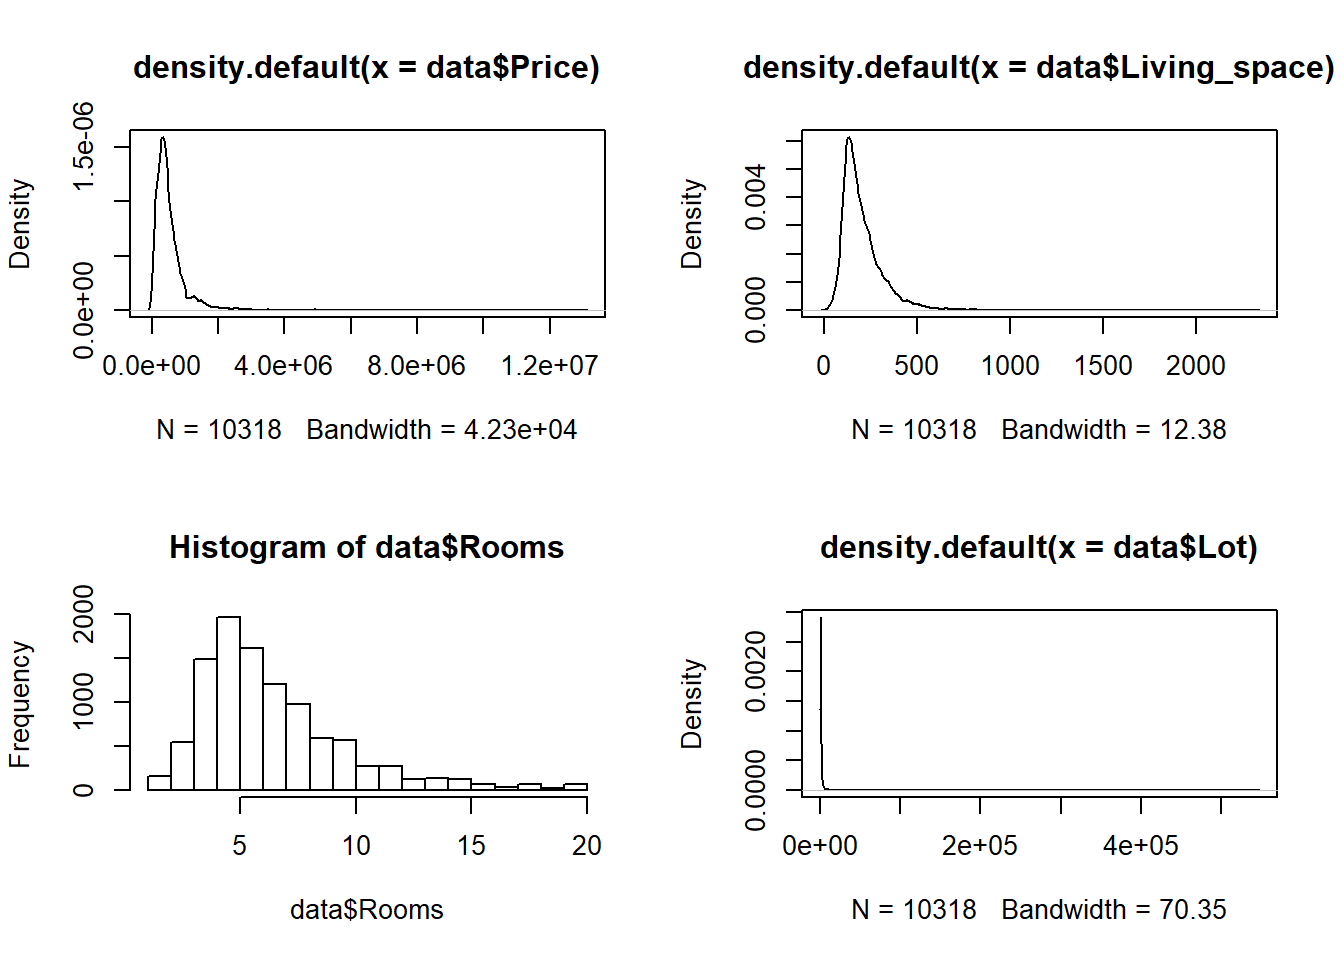
\includegraphics{Machine_Learning_Algorithms_Documentation_files/figure-latex/unnamed-chunk-3-1.pdf}

Result: The variables are right skewed

\textbf{Log Transformation of variables}

Therefore we will use the Log Transformation of the variables `Price',
`Living\_space', `Rooms', `Lot' to get a nearly normal distribution
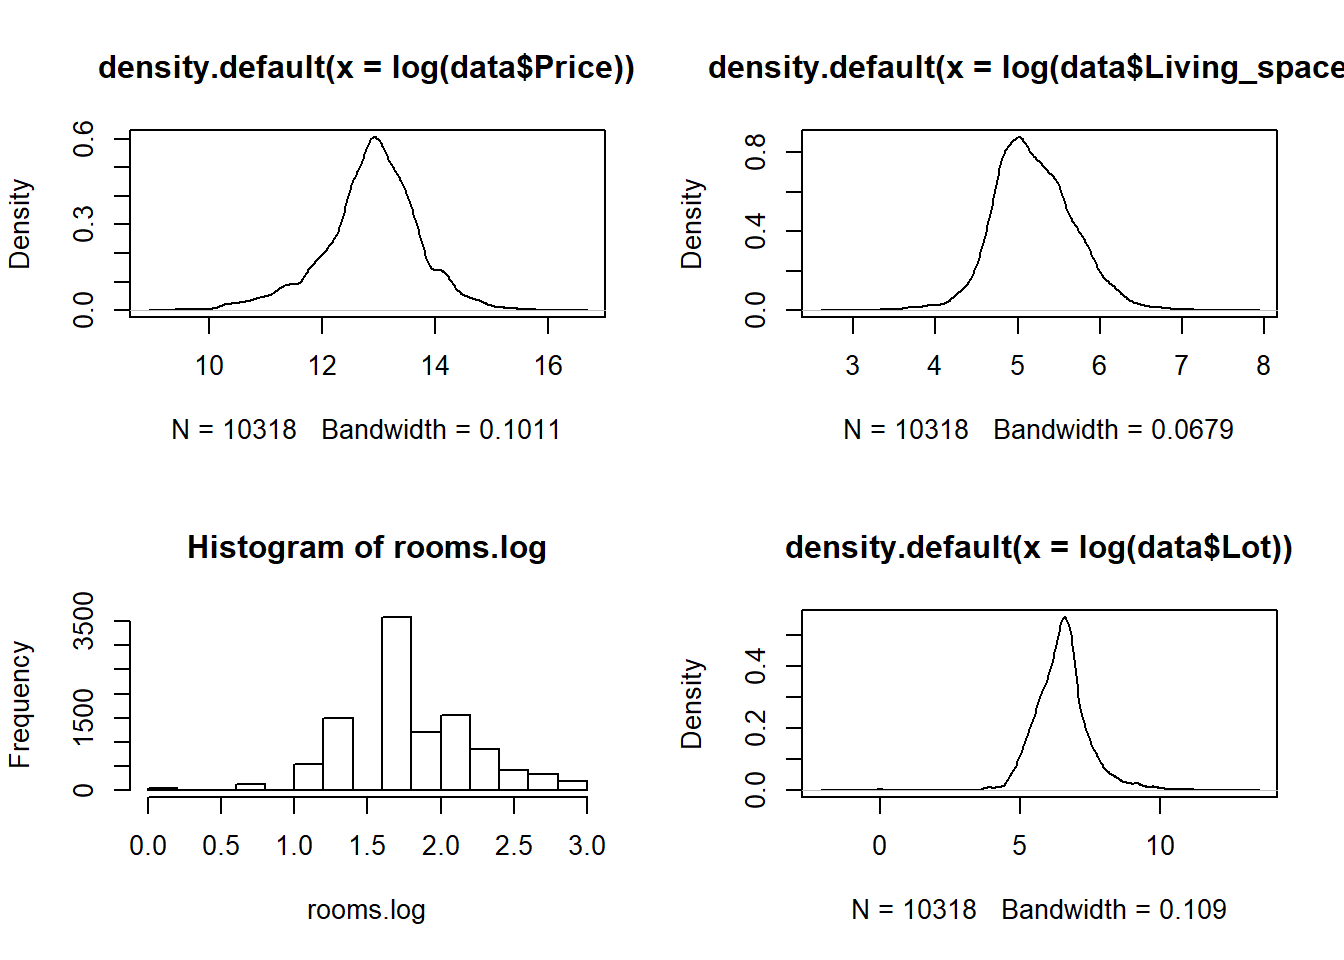
\includegraphics{Machine_Learning_Algorithms_Documentation_files/figure-latex/unnamed-chunk-4-1.pdf}

\textbf{Add new columns with log transformed variables price, living
space and rooms}

In order to easify access to the log transformed variables new columns
are created.

\begin{Shaded}
\begin{Highlighting}[]
\NormalTok{data1 <-}\StringTok{ }\NormalTok{data}
\NormalTok{data1}\OperatorTok{$}\NormalTok{log.price <-}\StringTok{ }\KeywordTok{log}\NormalTok{(data1}\OperatorTok{$}\NormalTok{Price)}
\NormalTok{data1}\OperatorTok{$}\NormalTok{log.living <-}\StringTok{ }\KeywordTok{log}\NormalTok{(data1}\OperatorTok{$}\NormalTok{Living_space)}
\NormalTok{data1}\OperatorTok{$}\NormalTok{log.rooms <-}\StringTok{ }\KeywordTok{log}\NormalTok{(data1}\OperatorTok{$}\NormalTok{Rooms)}
\NormalTok{data1}\OperatorTok{$}\NormalTok{log.lot <-}\StringTok{ }\KeywordTok{log}\NormalTok{(data1}\OperatorTok{$}\NormalTok{Lot)}
\end{Highlighting}
\end{Shaded}

\hypertarget{week-1---linear-models}{%
\section{Week 1 - Linear Models}\label{week-1---linear-models}}

\hypertarget{data-visualisation-and-linear-regressions}{%
\subsection{Data Visualisation and Linear
regressions}\label{data-visualisation-and-linear-regressions}}

\hypertarget{scatterplot-with-regression-line-for-logprice-against-logliving_space}{%
\subsection{Scatterplot with regression line for log(Price) against
log(Living\_space)}\label{scatterplot-with-regression-line-for-logprice-against-logliving_space}}

We plot the response variable ``Price'' against the predictor
``Living\_Space'' to get a first impression. The plot displays that
there is may a positive correlation between the two variables. We
further investigate this by a fitting a simple linear regression.
\includegraphics{Machine_Learning_Algorithms_Documentation_files/figure-latex/unnamed-chunk-7-1.pdf}

\hypertarget{fitting-a-simple-linear-regression-of-log.price-against-log.living-and-check-the-coefficients}{%
\subsection{Fitting a Simple Linear regression of log.price against
log.living and check the
coefficients}\label{fitting-a-simple-linear-regression-of-log.price-against-log.living-and-check-the-coefficients}}

\begin{Shaded}
\begin{Highlighting}[]
\CommentTok{#linear model}
\NormalTok{lm.log.price_living <-}\StringTok{ }\KeywordTok{lm}\NormalTok{(log.price }\OperatorTok{~}\StringTok{ }\NormalTok{log.living, }\DataTypeTok{data =}\NormalTok{ data1)}
\KeywordTok{summary}\NormalTok{(lm.log.price_living)}
\end{Highlighting}
\end{Shaded}

\begin{verbatim}
## 
## Call:
## lm(formula = log.price ~ log.living, data = data1)
## 
## Residuals:
##     Min      1Q  Median      3Q     Max 
## -3.7836 -0.4079  0.0856  0.4683  2.7581 
## 
## Coefficients:
##             Estimate Std. Error t value            Pr(>|t|)    
## (Intercept)  8.17522    0.07596  107.62 <0.0000000000000002 ***
## log.living   0.90280    0.01455   62.05 <0.0000000000000002 ***
## ---
## Signif. codes:  0 '***' 0.001 '**' 0.01 '*' 0.05 '.' 0.1 ' ' 1
## 
## Residual standard error: 0.7145 on 10316 degrees of freedom
## Multiple R-squared:  0.2718, Adjusted R-squared:  0.2717 
## F-statistic:  3850 on 1 and 10316 DF,  p-value: < 0.00000000000000022
\end{verbatim}

\begin{Shaded}
\begin{Highlighting}[]
\CommentTok{#estimated regression coefficients including p-values}
\KeywordTok{coef}\NormalTok{(lm.log.price_living)}
\end{Highlighting}
\end{Shaded}

\begin{verbatim}
## (Intercept)  log.living 
##   8.1752232   0.9028032
\end{verbatim}

\begin{Shaded}
\begin{Highlighting}[]
\KeywordTok{exp}\NormalTok{(}\KeywordTok{coef}\NormalTok{(lm.log.price_living))}
\end{Highlighting}
\end{Shaded}

\begin{verbatim}
## (Intercept)  log.living 
## 3551.847713    2.466508
\end{verbatim}

Result: very significant p-values for log.price \textasciitilde{}
log.living. We can assume that the variable log.living has an effect on
the dependent variable log.price with a positive correlation, meaning:
if the log.living parameter increases in value also the Price of the
property will increase.

Due to the log transformation of the variables we have to exponentiate
the values before the interpretation. For the intercept exp(8.17522)=
3551.84 and the slope exp(0.9028)=2.47, looking the p-values, which are
very small, we have a strong evidence that the slope of log.living is
not flat and therefore the variable has an effect on the log.price
variable.

\hypertarget{linear-regression-of-log.price-against-log.living-including-the-type-and-finding-the-intercept-for-the-different-types}{%
\subsection{Linear regression of log.price against log.living including
the Type and finding the intercept for the different
Types}\label{linear-regression-of-log.price-against-log.living-including-the-type-and-finding-the-intercept-for-the-different-types}}

\begin{Shaded}
\begin{Highlighting}[]
\CommentTok{##linear model}
\NormalTok{lm.log.price_living_type <-}\StringTok{ }\KeywordTok{lm}\NormalTok{(}\DataTypeTok{data =}\NormalTok{ data1, log.price }\OperatorTok{~}\StringTok{ }\NormalTok{log.living }\OperatorTok{+}\StringTok{ }\NormalTok{Type)}
\KeywordTok{summary}\NormalTok{(lm.log.price_living_type)}
\end{Highlighting}
\end{Shaded}

\begin{verbatim}
## 
## Call:
## lm(formula = log.price ~ log.living + Type, data = data1)
## 
## Residuals:
##     Min      1Q  Median      3Q     Max 
## -3.9802 -0.3849  0.0716  0.4556  2.7356 
## 
## Coefficients:
##                          Estimate Std. Error t value             Pr(>|t|)    
## (Intercept)               7.47225    0.09409  79.414 < 0.0000000000000002 ***
## log.living                0.99691    0.01679  59.378 < 0.0000000000000002 ***
## TypeBungalow              0.24691    0.05737   4.304    0.000016956457415 ***
## TypeCastle               -0.33356    0.31169  -1.070             0.284573    
## TypeCorner house         -0.14759    0.06058  -2.436             0.014857 *  
## TypeDuplex               -0.06320    0.03900  -1.620             0.105186    
## TypeFarmhouse             0.26026    0.04599   5.659    0.000000015603919 ***
## TypeMid-terrace house     0.24470    0.03679   6.651    0.000000000030494 ***
## TypeMultiple dwelling     0.35983    0.05029   7.155    0.000000000000891 ***
## TypeResidential property  0.17411    0.05094   3.418             0.000634 ***
## TypeSingle dwelling       0.39721    0.04091   9.708 < 0.0000000000000002 ***
## TypeSpecial property      0.46909    0.05103   9.193 < 0.0000000000000002 ***
## TypeVilla                 0.70309    0.05077  13.847 < 0.0000000000000002 ***
## ---
## Signif. codes:  0 '***' 0.001 '**' 0.01 '*' 0.05 '.' 0.1 ' ' 1
## 
## Residual standard error: 0.6912 on 10305 degrees of freedom
## Multiple R-squared:  0.3193, Adjusted R-squared:  0.3185 
## F-statistic: 402.8 on 12 and 10305 DF,  p-value: < 0.00000000000000022
\end{verbatim}

Result: due to the small p-values of the intercept and of the different
types we have a strong evidence that the different types have an effect
on the log.price \textasciitilde{} log.living. Only Type `Castle' and
Type `Duplex' seem not having an effect. Because of the log
transformation of the independent and dependent variables we have to
interpret an increase of living space by 1\% with an increase of the
price variable by about 0.99\% (according to the slope). The coefficient
of log.living is the estimated elasticity of price with respect to
living space.

\hypertarget{linear-regression-of-log.price-against-log.living-including-the-type-interaction}{%
\subsection{Linear regression of log.price against log.living including
the `Type'
interaction}\label{linear-regression-of-log.price-against-log.living-including-the-type-interaction}}

\begin{Shaded}
\begin{Highlighting}[]
\CommentTok{##linear model}
\NormalTok{lm.log.price_living_type2 <-}\StringTok{ }\KeywordTok{lm}\NormalTok{(}\DataTypeTok{data =}\NormalTok{ data1, log.price }\OperatorTok{~}\StringTok{ }\NormalTok{log.living }\OperatorTok{*}\StringTok{ }\NormalTok{Type)}
\end{Highlighting}
\end{Shaded}

\textbf{Measures of fit}

\begin{Shaded}
\begin{Highlighting}[]
\KeywordTok{formula}\NormalTok{(lm.log.price_living_type)}
\end{Highlighting}
\end{Shaded}

\begin{verbatim}
## log.price ~ log.living + Type
\end{verbatim}

\begin{Shaded}
\begin{Highlighting}[]
\CommentTok{#r.squared}
\KeywordTok{summary}\NormalTok{(lm.log.price_living_type)}\OperatorTok{$}\NormalTok{r.squared}
\end{Highlighting}
\end{Shaded}

\begin{verbatim}
## [1] 0.3192727
\end{verbatim}

\begin{Shaded}
\begin{Highlighting}[]
\CommentTok{#adj.r.squared}
\KeywordTok{summary}\NormalTok{(lm.log.price_living_type)}\OperatorTok{$}\NormalTok{adj.r.squared}
\end{Highlighting}
\end{Shaded}

\begin{verbatim}
## [1] 0.31848
\end{verbatim}

\begin{Shaded}
\begin{Highlighting}[]
\KeywordTok{formula}\NormalTok{(lm.log.price_living_type2)}
\end{Highlighting}
\end{Shaded}

\begin{verbatim}
## log.price ~ log.living * Type
\end{verbatim}

\begin{Shaded}
\begin{Highlighting}[]
\CommentTok{#r.squared}
\KeywordTok{summary}\NormalTok{(lm.log.price_living_type2)}\OperatorTok{$}\NormalTok{r.squared}
\end{Highlighting}
\end{Shaded}

\begin{verbatim}
## [1] 0.3263949
\end{verbatim}

\begin{Shaded}
\begin{Highlighting}[]
\CommentTok{#adj.r.squared}
\KeywordTok{summary}\NormalTok{(lm.log.price_living_type2)}\OperatorTok{$}\NormalTok{adj.r.squared}
\end{Highlighting}
\end{Shaded}

\begin{verbatim}
## [1] 0.3248899
\end{verbatim}

If we compare the R\^{}2 and adj. R\^{}2 of the additive and the
multiplicative model (for interaction), we see only a little
improvement. Therefore we might have to decide to continue with the less
complex model.

\hypertarget{fitted-values}{%
\subsection{Fitted values}\label{fitted-values}}

The function fitted() can be used to extract the predicted values for
the existing observations

\hypertarget{residuals-of-model-logprice-logliving_space}{%
\subsection{Residuals of model log(Price) \textasciitilde{}
log(Living\_space)}\label{residuals-of-model-logprice-logliving_space}}

\begin{Shaded}
\begin{Highlighting}[]
\KeywordTok{attach}\NormalTok{(data1)}
\NormalTok{resid.price_living <-}\StringTok{ }\KeywordTok{resid}\NormalTok{(lm.log.price_living)}
\KeywordTok{length}\NormalTok{(resid.price_living)}
\end{Highlighting}
\end{Shaded}

\begin{verbatim}
## [1] 10318
\end{verbatim}

\begin{Shaded}
\begin{Highlighting}[]
\KeywordTok{set.seed}\NormalTok{(}\DecValTok{100}\NormalTok{)}
\NormalTok{id <-}\StringTok{ }\KeywordTok{sample}\NormalTok{(}\DataTypeTok{x =} \DecValTok{1}\OperatorTok{:}\DecValTok{10318}\NormalTok{, }\DataTypeTok{size =} \DecValTok{5}\NormalTok{)}
\NormalTok{resid.price_living[id]}
\end{Highlighting}
\end{Shaded}

\begin{verbatim}
##       3786        503       3430       3696       4090 
##  0.5106768 -0.3315001  0.4470366 -0.9261093  1.0834033
\end{verbatim}

\begin{Shaded}
\begin{Highlighting}[]
\NormalTok{fitted.price_living[id]}
\end{Highlighting}
\end{Shaded}

\begin{verbatim}
##     3786      503     3430     3696     4090 
## 13.77484 12.69884 13.46378 12.41883 13.03221
\end{verbatim}

\begin{Shaded}
\begin{Highlighting}[]
\KeywordTok{plot}\NormalTok{(}\KeywordTok{log}\NormalTok{(Price) }\OperatorTok{~}\StringTok{ }\KeywordTok{log}\NormalTok{(Living_space), }\DataTypeTok{main =} \StringTok{'Model log(Price) ~ log(Living_space)'}\NormalTok{, }\DataTypeTok{col =} \StringTok{'navy'}\NormalTok{, }\DataTypeTok{pch =} \DecValTok{16}\NormalTok{)}
\KeywordTok{abline}\NormalTok{(lm.log.price_living, }\DataTypeTok{col =} \StringTok{'green'}\NormalTok{, }\DataTypeTok{lwd =} \FloatTok{2.5}\NormalTok{)}
\KeywordTok{points}\NormalTok{(}\KeywordTok{log}\NormalTok{(Price) }\OperatorTok{~}\StringTok{ }\KeywordTok{log}\NormalTok{(Living_space), }\DataTypeTok{data =}\NormalTok{ data1[id, ], }\DataTypeTok{col =} \StringTok{'red'}\NormalTok{, }\DataTypeTok{pch =} \DecValTok{4}\NormalTok{, }\DataTypeTok{lwd =} \DecValTok{5}\NormalTok{)}
\KeywordTok{segments}\NormalTok{(}\DataTypeTok{x0 =}\NormalTok{ data1[id, }\StringTok{'log.living'}\NormalTok{], }\DataTypeTok{x1 =}\NormalTok{ data1[id, }\StringTok{'log.living'}\NormalTok{],}
         \DataTypeTok{y0 =}\NormalTok{ fitted.price_living[id], }\DataTypeTok{y1 =}\NormalTok{ data1[id, }\StringTok{'log.price'}\NormalTok{], }\DataTypeTok{col =} \StringTok{'yellow'}\NormalTok{, }\DataTypeTok{lwd =} \DecValTok{2}\NormalTok{)}
\end{Highlighting}
\end{Shaded}

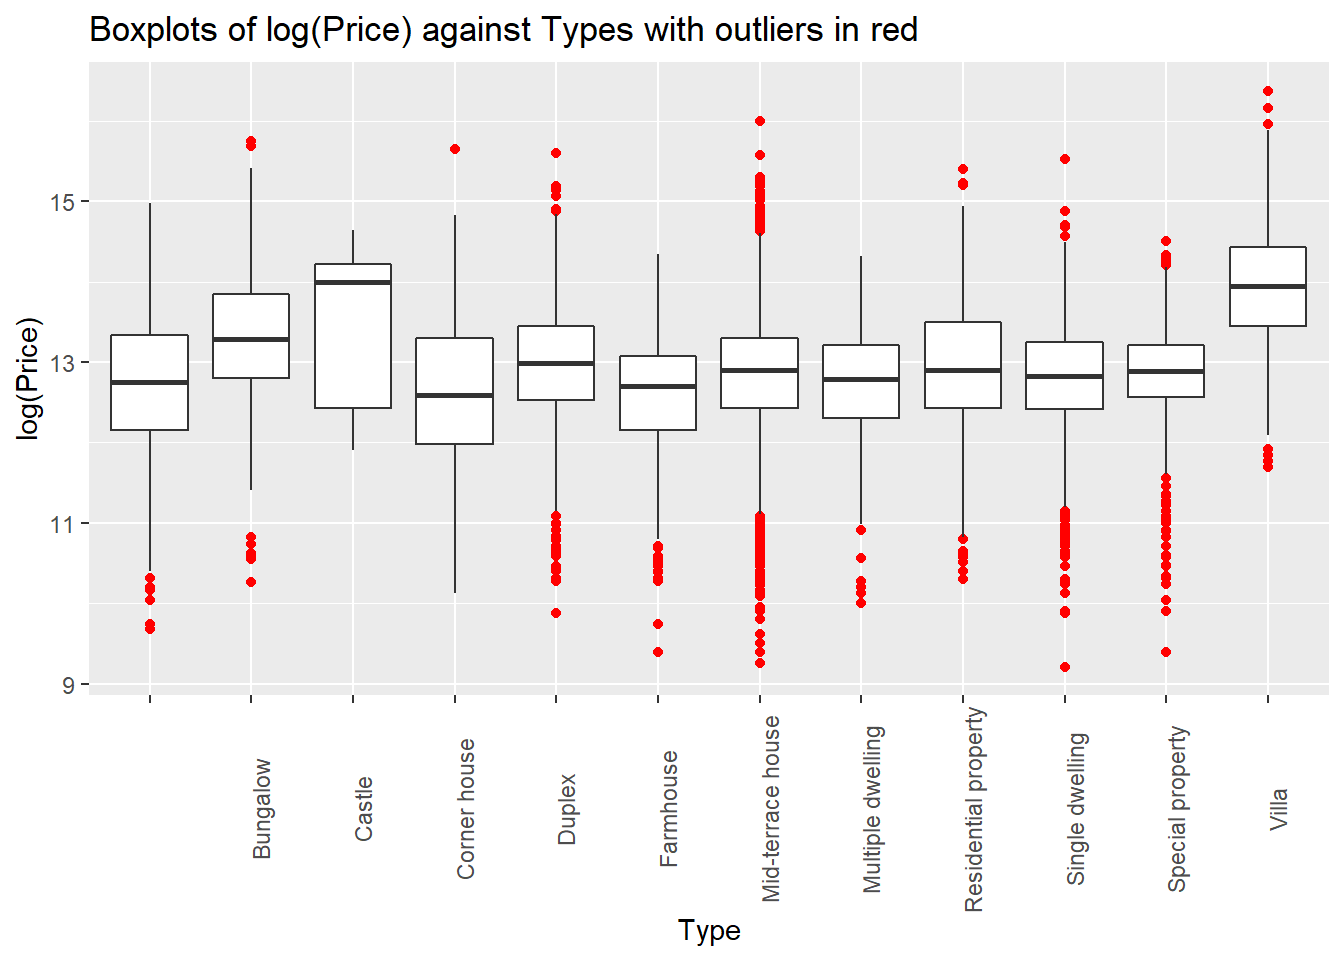
\includegraphics{Machine_Learning_Algorithms_Documentation_files/figure-latex/unnamed-chunk-14-1.pdf}

With this code we take 5 examples of the data set and plot it with the
predicted values including the residuals (yellow line), which indicates
the distance to the estimated regression line.

\hypertarget{predicting-values-using-splitted-data-set-991-ratio}{%
\subsection{Predicting values using splitted data set 99:1
ratio}\label{predicting-values-using-splitted-data-set-991-ratio}}

\begin{Shaded}
\begin{Highlighting}[]
\CommentTok{#split dataset }
\NormalTok{split99 <-}\StringTok{ }\KeywordTok{round}\NormalTok{(}\KeywordTok{nrow}\NormalTok{(data1)}\OperatorTok{*}\StringTok{ }\FloatTok{0.99}\NormalTok{)}
\NormalTok{train <-}\StringTok{ }\NormalTok{data1[}\DecValTok{1}\OperatorTok{:}\NormalTok{split99,]}
\NormalTok{test <-}\StringTok{ }\NormalTok{data1[(split99 }\OperatorTok{+}\StringTok{ }\DecValTok{1}\NormalTok{)}\OperatorTok{:}\KeywordTok{nrow}\NormalTok{(data1),]}
\CommentTok{#linear regression model}
\NormalTok{lm.train <-}\StringTok{ }\KeywordTok{lm}\NormalTok{(log.price }\OperatorTok{~}\StringTok{ }\NormalTok{log.living, }\DataTypeTok{data =}\NormalTok{ train)}
\KeywordTok{summary}\NormalTok{(lm.train)}
\end{Highlighting}
\end{Shaded}

\begin{verbatim}
## 
## Call:
## lm(formula = log.price ~ log.living, data = train)
## 
## Residuals:
##     Min      1Q  Median      3Q     Max 
## -3.7888 -0.4043  0.0847  0.4633  2.7534 
## 
## Coefficients:
##             Estimate Std. Error t value            Pr(>|t|)    
## (Intercept)  8.19143    0.07604  107.72 <0.0000000000000002 ***
## log.living   0.90074    0.01456   61.84 <0.0000000000000002 ***
## ---
## Signif. codes:  0 '***' 0.001 '**' 0.01 '*' 0.05 '.' 0.1 ' ' 1
## 
## Residual standard error: 0.711 on 10213 degrees of freedom
## Multiple R-squared:  0.2725, Adjusted R-squared:  0.2724 
## F-statistic:  3825 on 1 and 10213 DF,  p-value: < 0.00000000000000022
\end{verbatim}

\begin{Shaded}
\begin{Highlighting}[]
\CommentTok{#predictions}
\NormalTok{pred.new.living <-}\StringTok{ }\KeywordTok{predict}\NormalTok{(}\DataTypeTok{object =}\NormalTok{ lm.train, }\DataTypeTok{newdata =}\NormalTok{ test)}
\NormalTok{pred.new.living.CI <-}\StringTok{ }\KeywordTok{predict}\NormalTok{(}\DataTypeTok{object =}\NormalTok{ lm.train, }\DataTypeTok{interval =} \StringTok{'prediction'}\NormalTok{, }\DataTypeTok{newdata =}\NormalTok{ test)}

\KeywordTok{plot}\NormalTok{(log.price }\OperatorTok{~}\StringTok{ }\NormalTok{log.living, }\DataTypeTok{data =}\NormalTok{ train, }\DataTypeTok{main =} \StringTok{'Prediction with Model log(Price) ~ log(Living_space)'}\NormalTok{, }\DataTypeTok{col =} \StringTok{'navy'}\NormalTok{, }\DataTypeTok{pch =} \DecValTok{16}\NormalTok{)}
\KeywordTok{segments}\NormalTok{(}\DataTypeTok{x0 =}\NormalTok{ test}\OperatorTok{$}\NormalTok{log.living, }\DataTypeTok{x1 =}\NormalTok{ test}\OperatorTok{$}\NormalTok{log.living,}
         \DataTypeTok{y0 =}\NormalTok{ pred.new.living.CI[, }\StringTok{'lwr'}\NormalTok{], }\DataTypeTok{y1 =}\NormalTok{ pred.new.living.CI[, }\StringTok{'upr'}\NormalTok{], }\DataTypeTok{lwd =} \DecValTok{2}\NormalTok{, }\DataTypeTok{col =} \StringTok{'green'}\NormalTok{)}
\KeywordTok{points}\NormalTok{(}\DataTypeTok{x =}\NormalTok{ test}\OperatorTok{$}\NormalTok{log.living, }\DataTypeTok{y=}\NormalTok{ pred.new.living.CI[,}\StringTok{'fit'}\NormalTok{], }\DataTypeTok{col =} \StringTok{'red'}\NormalTok{, }\DataTypeTok{pch =} \DecValTok{16}\NormalTok{, }\DataTypeTok{cex =}\FloatTok{1.5}\NormalTok{)}
\KeywordTok{abline}\NormalTok{(lm.train, }\DataTypeTok{col =} \StringTok{'yellow'}\NormalTok{, }\DataTypeTok{lwd =} \FloatTok{2.5}\NormalTok{)}
\end{Highlighting}
\end{Shaded}

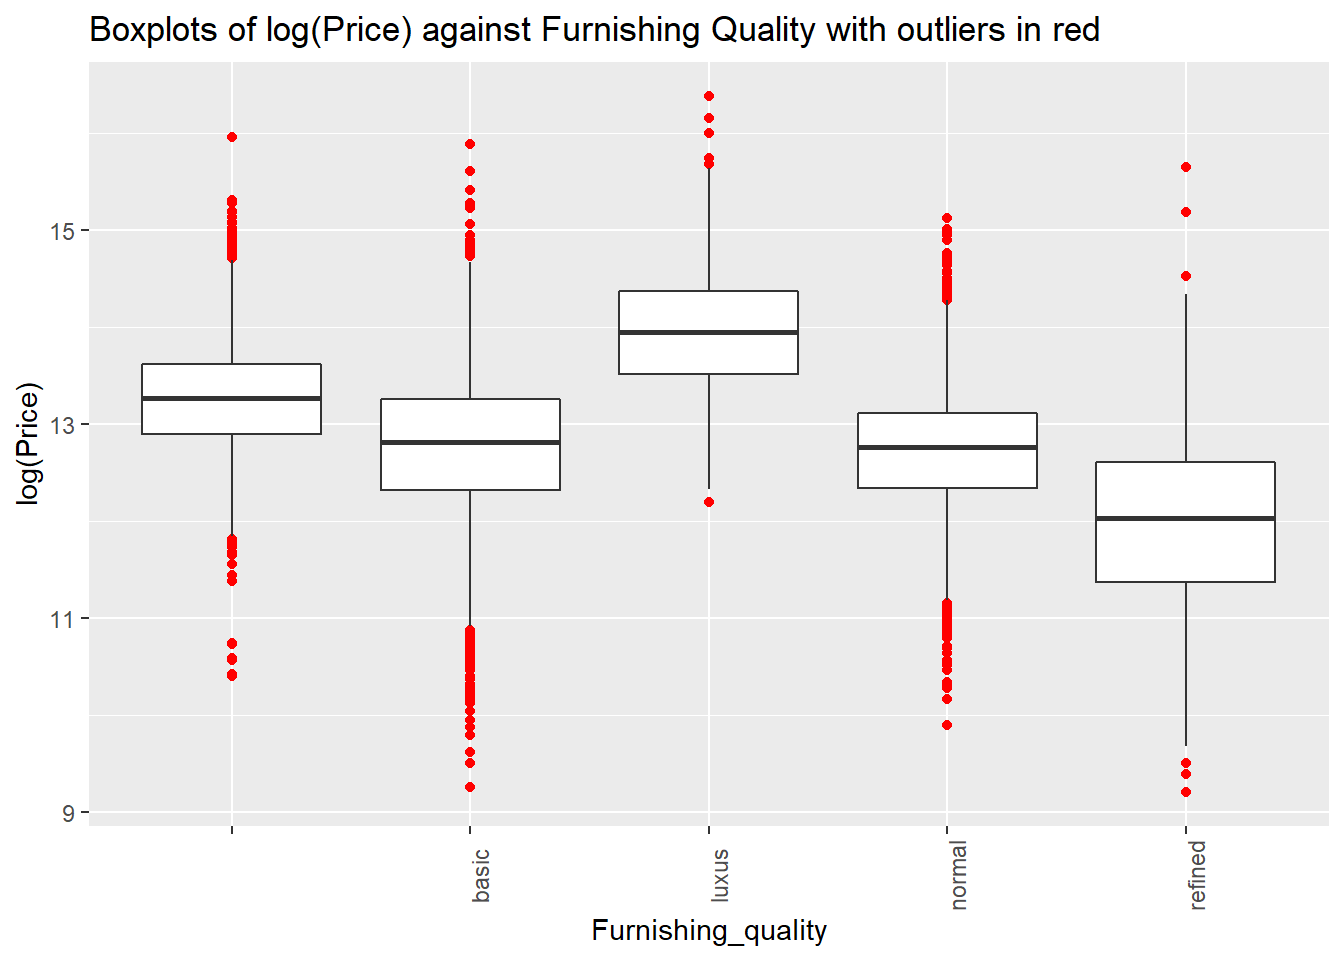
\includegraphics{Machine_Learning_Algorithms_Documentation_files/figure-latex/unnamed-chunk-15-1.pdf}

In this plot we see the estimated regression line (in yellow) with the
estimated values (red dots) with the corresponding confident interval
(green lines). The blue dots are the original dataset points.

\hypertarget{testing-the-effect-of-a-categorical-variable-and-post-hoc-contrasts}{%
\subsection{Testing the effect of a categorical variable and post-hoc
contrasts}\label{testing-the-effect-of-a-categorical-variable-and-post-hoc-contrasts}}

\begin{Shaded}
\begin{Highlighting}[]
\NormalTok{condition.box.with_outlier <-}\StringTok{ }\KeywordTok{ggplot}\NormalTok{(data1, }\KeywordTok{aes}\NormalTok{(}\DataTypeTok{x=}\NormalTok{Condition, }\DataTypeTok{y=}\NormalTok{log.price)) }\OperatorTok{+}\StringTok{ }\KeywordTok{geom_boxplot}\NormalTok{(}\DataTypeTok{outlier.colour =} \StringTok{'red'}\NormalTok{)}\OperatorTok{+}\StringTok{ }\KeywordTok{theme}\NormalTok{(}\DataTypeTok{axis.text.x =} \KeywordTok{element_text}\NormalTok{(}\DataTypeTok{angle =} \DecValTok{90}\NormalTok{)) }\OperatorTok{+}\StringTok{ }\KeywordTok{ggtitle}\NormalTok{(}\StringTok{'Boxplots of log(Price) against Condition with outliers in red'}\NormalTok{)}
\KeywordTok{plot}\NormalTok{(condition.box.with_outlier)}
\end{Highlighting}
\end{Shaded}

\includegraphics{Machine_Learning_Algorithms_Documentation_files/figure-latex/unnamed-chunk-16-1.pdf}

\begin{Shaded}
\begin{Highlighting}[]
\CommentTok{#model}
\NormalTok{lm.price_condition}\FloatTok{.1}\NormalTok{ <-}\StringTok{ }\KeywordTok{lm}\NormalTok{(log.price }\OperatorTok{~}\StringTok{ }\NormalTok{Condition, }\DataTypeTok{data =}\NormalTok{ data1)}
\KeywordTok{summary}\NormalTok{(lm.price_condition}\FloatTok{.1}\NormalTok{)}
\end{Highlighting}
\end{Shaded}

\begin{verbatim}
## 
## Call:
## lm(formula = log.price ~ Condition, data = data1)
## 
## Residuals:
##     Min      1Q  Median      3Q     Max 
## -3.6043 -0.4304  0.0333  0.4884  3.6247 
## 
## Coefficients:
##                                               Estimate Std. Error t value
## (Intercept)                                   12.95695    0.04213 307.553
## Conditionas new                               -1.01885    0.24696  -4.126
## Conditiondilapidated                           0.47108    0.04838   9.738
## Conditionfirst occupation                      0.19331    0.09330   2.072
## Conditionfirst occupation after refurbishment -0.05091    0.05685  -0.895
## Conditionfixer-upper                          -0.10881    0.05398  -2.016
## Conditionmaintained                           -0.42435    0.04906  -8.649
## Conditionrefurbished                          -0.14229    0.04328  -3.288
##                                                           Pr(>|t|)    
## (Intercept)                                   < 0.0000000000000002 ***
## Conditionas new                                          0.0000373 ***
## Conditiondilapidated                          < 0.0000000000000002 ***
## Conditionfirst occupation                                  0.03829 *  
## Conditionfirst occupation after refurbishment              0.37055    
## Conditionfixer-upper                                       0.04384 *  
## Conditionmaintained                           < 0.0000000000000002 ***
## Conditionrefurbished                                       0.00101 ** 
## ---
## Signif. codes:  0 '***' 0.001 '**' 0.01 '*' 0.05 '.' 0.1 ' ' 1
## 
## Residual standard error: 0.8071 on 10310 degrees of freedom
## Multiple R-squared:  0.07146,    Adjusted R-squared:  0.07083 
## F-statistic: 113.4 on 7 and 10310 DF,  p-value: < 0.00000000000000022
\end{verbatim}

\begin{Shaded}
\begin{Highlighting}[]
\CommentTok{#coefficients}
\KeywordTok{coef}\NormalTok{(lm.price_condition}\FloatTok{.1}\NormalTok{)}
\end{Highlighting}
\end{Shaded}

\begin{verbatim}
##                                   (Intercept) 
##                                   12.95694626 
##                               Conditionas new 
##                                   -1.01884973 
##                          Conditiondilapidated 
##                                    0.47108462 
##                     Conditionfirst occupation 
##                                    0.19330741 
## Conditionfirst occupation after refurbishment 
##                                   -0.05090966 
##                          Conditionfixer-upper 
##                                   -0.10881029 
##                           Conditionmaintained 
##                                   -0.42434950 
##                          Conditionrefurbished 
##                                   -0.14228677
\end{verbatim}

\begin{Shaded}
\begin{Highlighting}[]
\KeywordTok{aggregate}\NormalTok{(log.price }\OperatorTok{~}\NormalTok{Condition, }
          \DataTypeTok{FUN =}\NormalTok{ mean, }\DataTypeTok{data =}\NormalTok{ data1)}
\end{Highlighting}
\end{Shaded}

\begin{verbatim}
##                              Condition log.price
## 1                                       12.95695
## 2                               as new  11.93810
## 3                          dilapidated  13.42803
## 4                     first occupation  13.15025
## 5 first occupation after refurbishment  12.90604
## 6                          fixer-upper  12.84814
## 7                           maintained  12.53260
## 8                          refurbished  12.81466
\end{verbatim}

\begin{Shaded}
\begin{Highlighting}[]
\CommentTok{#model without slope, only intercept}
\NormalTok{lm.price_condition}\FloatTok{.0}\NormalTok{ <-}\StringTok{ }\KeywordTok{lm}\NormalTok{(log.price }\OperatorTok{~}\StringTok{ }\DecValTok{1}\NormalTok{, }\DataTypeTok{data =}\NormalTok{ data1)}
\KeywordTok{summary}\NormalTok{(lm.price_condition}\FloatTok{.0}\NormalTok{)}
\end{Highlighting}
\end{Shaded}

\begin{verbatim}
## 
## Call:
## lm(formula = log.price ~ 1, data = data1)
## 
## Residuals:
##     Min      1Q  Median      3Q     Max 
## -3.6576 -0.4388  0.0287  0.5166  3.5125 
## 
## Coefficients:
##              Estimate Std. Error t value            Pr(>|t|)    
## (Intercept) 12.867983   0.008243    1561 <0.0000000000000002 ***
## ---
## Signif. codes:  0 '***' 0.001 '**' 0.01 '*' 0.05 '.' 0.1 ' ' 1
## 
## Residual standard error: 0.8373 on 10317 degrees of freedom
\end{verbatim}

\begin{Shaded}
\begin{Highlighting}[]
\KeywordTok{coef}\NormalTok{(lm.price_condition}\FloatTok{.0}\NormalTok{)}
\end{Highlighting}
\end{Shaded}

\begin{verbatim}
## (Intercept) 
##    12.86798
\end{verbatim}

\begin{Shaded}
\begin{Highlighting}[]
\CommentTok{#Anova}
\KeywordTok{anova}\NormalTok{(lm.price_condition}\FloatTok{.0}\NormalTok{, lm.price_condition}\FloatTok{.1}\NormalTok{)}
\end{Highlighting}
\end{Shaded}

\begin{verbatim}
## Analysis of Variance Table
## 
## Model 1: log.price ~ 1
## Model 2: log.price ~ Condition
##   Res.Df    RSS Df Sum of Sq      F                Pr(>F)    
## 1  10317 7232.5                                              
## 2  10310 6715.7  7    516.86 113.36 < 0.00000000000000022 ***
## ---
## Signif. codes:  0 '***' 0.001 '**' 0.01 '*' 0.05 '.' 0.1 ' ' 1
\end{verbatim}

\begin{Shaded}
\begin{Highlighting}[]
\CommentTok{#post-hoc contrasts}
\KeywordTok{library}\NormalTok{(multcomp)}
\NormalTok{ph.test}\FloatTok{.1}\NormalTok{ <-}\StringTok{ }\KeywordTok{glht}\NormalTok{(}\DataTypeTok{model =}\NormalTok{ lm.price_condition}\FloatTok{.1}\NormalTok{, }\DataTypeTok{linfct =} \KeywordTok{mcp}\NormalTok{(}\DataTypeTok{Condition =} \KeywordTok{c}\NormalTok{(}\StringTok{'refurbished - dilapidated = 0'}\NormalTok{)))}
\KeywordTok{summary}\NormalTok{(ph.test}\FloatTok{.1}\NormalTok{)}
\end{Highlighting}
\end{Shaded}

\begin{verbatim}
## 
##   Simultaneous Tests for General Linear Hypotheses
## 
## Multiple Comparisons of Means: User-defined Contrasts
## 
## 
## Fit: lm(formula = log.price ~ Condition, data = data1)
## 
## Linear Hypotheses:
##                                Estimate Std. Error t value            Pr(>|t|)
## refurbished - dilapidated == 0 -0.61337    0.02576  -23.81 <0.0000000000000002
##                                   
## refurbished - dilapidated == 0 ***
## ---
## Signif. codes:  0 '***' 0.001 '**' 0.01 '*' 0.05 '.' 0.1 ' ' 1
## (Adjusted p values reported -- single-step method)
\end{verbatim}

R uses ``treatment contrasts'' and therefore the Intercept refers to the
first in alphabetical order, here ``Null''. The other coefficients
represent the difference.

Whilst considering the boxplots, it seems rather suprising that `as new'
has the lowest mean price value.

Condition `as new', `dilapidated', `first occupation', `maintained' to
have a strong effect on the response variable. The results are very
suprising, as new condition negatively influences the price and
condition dilapidated increases the price.

The results obtained seem weak, represented in the adj. R-squared with
0.07083.

To further test the predictor an lm is built without slopes for every
type and then tested by an F-Test (Anova). Surprsingly, the Model with
slopes for the Type seems to perform better as indicated through a lower
RSS value.

The post-hoc contrasts is used to test whether `dilapidated' and
`refurbished' differ. The outcome states that `dilapidated' increases
the price. This confirms also the visual analysis of the boxplots, but
still is suprising as explained above.

\hypertarget{adding-more-categorical-variables-to-the-testing-above}{%
\subsection{Adding more categorical variables to the testing
above}\label{adding-more-categorical-variables-to-the-testing-above}}

\begin{Shaded}
\begin{Highlighting}[]
\NormalTok{Year_built1 <-}\StringTok{ }\KeywordTok{as.integer}\NormalTok{(data1}\OperatorTok{$}\NormalTok{Year_built)}
\NormalTok{floor1 <-}\StringTok{ }\KeywordTok{as.integer}\NormalTok{(data1}\OperatorTok{$}\NormalTok{Floors)}
\KeywordTok{typeof}\NormalTok{(Year_built1)}
\end{Highlighting}
\end{Shaded}

\begin{verbatim}
## [1] "integer"
\end{verbatim}

\begin{Shaded}
\begin{Highlighting}[]
\NormalTok{lm.price_condition}\FloatTok{.2}\NormalTok{ <-}\StringTok{ }\KeywordTok{update}\NormalTok{(lm.price_condition}\FloatTok{.1}\NormalTok{,. }\OperatorTok{~}\StringTok{ }\NormalTok{. }\OperatorTok{+}\StringTok{ }\NormalTok{Type }\OperatorTok{+}\StringTok{ }\NormalTok{log.rooms }\OperatorTok{+}
\StringTok{                                 }\NormalTok{State }\OperatorTok{+}\StringTok{ }\NormalTok{Energy_efficiency_class }\OperatorTok{+}\StringTok{ }\NormalTok{Year_built1 }\OperatorTok{+}\StringTok{ }\NormalTok{Furnishing_quality }\OperatorTok{+}\StringTok{ }\NormalTok{floor1)}
\KeywordTok{formula}\NormalTok{(lm.price_condition}\FloatTok{.2}\NormalTok{)}
\end{Highlighting}
\end{Shaded}

\begin{verbatim}
## log.price ~ Condition + Type + log.rooms + State + Energy_efficiency_class + 
##     Year_built1 + Furnishing_quality + floor1
\end{verbatim}

\begin{Shaded}
\begin{Highlighting}[]
\KeywordTok{drop1}\NormalTok{(lm.price_condition}\FloatTok{.2}\NormalTok{, }\DataTypeTok{test =} \StringTok{"F"}\NormalTok{)}
\end{Highlighting}
\end{Shaded}

\begin{verbatim}
## Single term deletions
## 
## Model:
## log.price ~ Condition + Type + log.rooms + State + Energy_efficiency_class + 
##     Year_built1 + Furnishing_quality + floor1
##                         Df Sum of Sq    RSS     AIC  F value
## <none>                               2148.4 -8631.8         
## Condition                7     17.57 2165.9 -8587.1   8.3684
## Type                    11    134.63 2283.0 -8215.5  40.7950
## log.rooms                1    152.62 2301.0 -8138.9 508.7221
## State                   15    638.74 2787.1 -6784.8 141.9381
## Energy_efficiency_class  9     33.56 2181.9 -8538.0  12.4294
## Year_built1              1     56.88 2205.2 -8445.4 189.5786
## Furnishing_quality       4    346.08 2494.4 -7562.8 288.3902
## floor1                   1     31.86 2180.2 -8527.7 106.1896
##                                        Pr(>F)    
## <none>                                           
## Condition                     0.0000000003205 ***
## Type                    < 0.00000000000000022 ***
## log.rooms               < 0.00000000000000022 ***
## State                   < 0.00000000000000022 ***
## Energy_efficiency_class < 0.00000000000000022 ***
## Year_built1             < 0.00000000000000022 ***
## Furnishing_quality      < 0.00000000000000022 ***
## floor1                  < 0.00000000000000022 ***
## ---
## Signif. codes:  0 '***' 0.001 '**' 0.01 '*' 0.05 '.' 0.1 ' ' 1
\end{verbatim}

Drop1 function performes automatically or each variable presence in the
model an F test. According to the results all independent variables in
the model seem to have an effect.

\hypertarget{week-2---non-linearity}{%
\section{Week 2 - Non-linearity}\label{week-2---non-linearity}}

\hypertarget{polynomials}{%
\subsection{Polynomials}\label{polynomials}}

By including polynomials (e.g.~x1 + x1\^{}2) we can model non linear
relationships with a Linear Model.

\begin{Shaded}
\begin{Highlighting}[]
\KeywordTok{library}\NormalTok{(ggplot2)}
\KeywordTok{attach}\NormalTok{(data1)}
\end{Highlighting}
\end{Shaded}

\textbf{Graphical analysis}

log(Price) \textasciitilde{} log(Living\_space)

\begin{Shaded}
\begin{Highlighting}[]
\NormalTok{gg.log.price_log.living <-}\StringTok{ }\KeywordTok{ggplot}\NormalTok{(data1,}\DataTypeTok{mapping =} \KeywordTok{aes}\NormalTok{(}\DataTypeTok{y =}\NormalTok{ log.price, }\DataTypeTok{x =}\NormalTok{ log.living)) }\OperatorTok{+}\StringTok{ }\KeywordTok{geom_point}\NormalTok{()}
\NormalTok{gg.log.price_log.living }\OperatorTok{+}\StringTok{ }\KeywordTok{geom_smooth}\NormalTok{()}
\end{Highlighting}
\end{Shaded}

\begin{verbatim}
## `geom_smooth()` using method = 'gam' and formula 'y ~ s(x, bs = "cs")'
\end{verbatim}

\includegraphics{Machine_Learning_Algorithms_Documentation_files/figure-latex/unnamed-chunk-19-1.pdf}
The graphical analysis shows a non-linear relationship for the predictor
living\_space.

\#model with a linear effect for log.living with log.rooms

\begin{Shaded}
\begin{Highlighting}[]
\CommentTok{#model with a linear effect for log.living}
\NormalTok{lm.living}\FloatTok{.1}\NormalTok{ <-}\StringTok{ }\KeywordTok{lm}\NormalTok{(log.price }\OperatorTok{~}\StringTok{ }\NormalTok{log.living }\OperatorTok{+}\StringTok{ }\NormalTok{log.rooms)}
\KeywordTok{summary}\NormalTok{(lm.living}\FloatTok{.1}\NormalTok{)}
\end{Highlighting}
\end{Shaded}

\begin{verbatim}
## 
## Call:
## lm(formula = log.price ~ log.living + log.rooms)
## 
## Residuals:
##     Min      1Q  Median      3Q     Max 
## -3.9154 -0.3918  0.0788  0.4617  2.6939 
## 
## Coefficients:
##             Estimate Std. Error t value            Pr(>|t|)    
## (Intercept)  7.41210    0.08773   84.49 <0.0000000000000002 ***
## log.living   1.19671    0.02268   52.76 <0.0000000000000002 ***
## log.rooms   -0.41705    0.02492  -16.74 <0.0000000000000002 ***
## ---
## Signif. codes:  0 '***' 0.001 '**' 0.01 '*' 0.05 '.' 0.1 ' ' 1
## 
## Residual standard error: 0.7051 on 10315 degrees of freedom
## Multiple R-squared:  0.291,  Adjusted R-squared:  0.2909 
## F-statistic:  2117 on 2 and 10315 DF,  p-value: < 0.00000000000000022
\end{verbatim}

Both predictors show a strong effect on the response variable price. Now
we want to build a model with a quadratic effect for living space.

\#model with a cuadratic effect for log.living

\begin{Shaded}
\begin{Highlighting}[]
\CommentTok{#model with a quadratic poly}
\NormalTok{lm.living}\FloatTok{.2}\NormalTok{ <-}\StringTok{ }\KeywordTok{lm}\NormalTok{(log.price }\OperatorTok{~}\StringTok{ }\NormalTok{log.rooms }\OperatorTok{+}\StringTok{ }\KeywordTok{poly}\NormalTok{(log.living, }\DataTypeTok{degree =} \DecValTok{2}\NormalTok{))}
\KeywordTok{summary}\NormalTok{(lm.living}\FloatTok{.2}\NormalTok{)}
\end{Highlighting}
\end{Shaded}

\begin{verbatim}
## 
## Call:
## lm(formula = log.price ~ log.rooms + poly(log.living, degree = 2))
## 
## Residuals:
##     Min      1Q  Median      3Q     Max 
## -3.9761 -0.3927  0.0714  0.4552  2.6652 
## 
## Coefficients:
##                               Estimate Std. Error t value            Pr(>|t|)
## (Intercept)                   13.68390    0.04616  296.42 <0.0000000000000002
## log.rooms                     -0.44504    0.02490  -17.88 <0.0000000000000002
## poly(log.living, degree = 2)1 59.73564    1.11071   53.78 <0.0000000000000002
## poly(log.living, degree = 2)2 -7.82809    0.70453  -11.11 <0.0000000000000002
##                                  
## (Intercept)                   ***
## log.rooms                     ***
## poly(log.living, degree = 2)1 ***
## poly(log.living, degree = 2)2 ***
## ---
## Signif. codes:  0 '***' 0.001 '**' 0.01 '*' 0.05 '.' 0.1 ' ' 1
## 
## Residual standard error: 0.7009 on 10314 degrees of freedom
## Multiple R-squared:  0.2994, Adjusted R-squared:  0.2992 
## F-statistic:  1469 on 3 and 10314 DF,  p-value: < 0.00000000000000022
\end{verbatim}

Now that we have added the quadratic effect(with degree = 2). The two
models can be compared by an F-Test.

\#Compare the two models by an F-Test

\begin{Shaded}
\begin{Highlighting}[]
\CommentTok{#test in quadratic}
\KeywordTok{anova}\NormalTok{(lm.living}\FloatTok{.1}\NormalTok{, lm.living}\FloatTok{.2}\NormalTok{)}
\end{Highlighting}
\end{Shaded}

\begin{verbatim}
## Analysis of Variance Table
## 
## Model 1: log.price ~ log.living + log.rooms
## Model 2: log.price ~ log.rooms + poly(log.living, degree = 2)
##   Res.Df    RSS Df Sum of Sq      F                Pr(>F)    
## 1  10315 5127.7                                              
## 2  10314 5067.1  1    60.652 123.46 < 0.00000000000000022 ***
## ---
## Signif. codes:  0 '***' 0.001 '**' 0.01 '*' 0.05 '.' 0.1 ' ' 1
\end{verbatim}

The second model with a quadratic effect for living space has a better
performance, as the RSS is lower than the one from the model without a
quadratic effect. Additionally, the p-value indicates that the second
model performs better.

\begin{Shaded}
\begin{Highlighting}[]
\CommentTok{#plot}
\NormalTok{gg.log.price_log.living }\OperatorTok{+}\StringTok{ }\KeywordTok{geom_smooth}\NormalTok{(}\DataTypeTok{method =} \StringTok{'lm'}\NormalTok{, }\DataTypeTok{formula =}\NormalTok{ y }\OperatorTok{~}\KeywordTok{poly}\NormalTok{(x, }\DataTypeTok{degree =} \DecValTok{2}\NormalTok{))}
\end{Highlighting}
\end{Shaded}

\includegraphics{Machine_Learning_Algorithms_Documentation_files/figure-latex/unnamed-chunk-23-1.pdf}

The quadratic fit seems to model the non-linear relationship of living
space quite well. Nevertheless, we try to fit a cubic poly.

\#model with a cubic poly

\begin{Shaded}
\begin{Highlighting}[]
\CommentTok{#model with a cubic poly}
\NormalTok{lm.living}\FloatTok{.3}\NormalTok{ <-}\StringTok{ }\KeywordTok{lm}\NormalTok{(log.price }\OperatorTok{~}\StringTok{ }\NormalTok{log.rooms }\OperatorTok{+}\StringTok{ }\KeywordTok{poly}\NormalTok{(log.living, }\DataTypeTok{degree =} \DecValTok{3}\NormalTok{))}
\KeywordTok{summary}\NormalTok{(lm.living}\FloatTok{.3}\NormalTok{)}
\end{Highlighting}
\end{Shaded}

\begin{verbatim}
## 
## Call:
## lm(formula = log.price ~ log.rooms + poly(log.living, degree = 3))
## 
## Residuals:
##     Min      1Q  Median      3Q     Max 
## -3.9763 -0.3928  0.0714  0.4553  2.6650 
## 
## Coefficients:
##                               Estimate Std. Error t value            Pr(>|t|)
## (Intercept)                   13.68416    0.04669 293.108 <0.0000000000000002
## log.rooms                     -0.44519    0.02519 -17.676 <0.0000000000000002
## poly(log.living, degree = 3)1 59.74067    1.11848  53.412 <0.0000000000000002
## poly(log.living, degree = 3)2 -7.82850    0.70465 -11.110 <0.0000000000000002
## poly(log.living, degree = 3)3 -0.02715    0.70903  -0.038               0.969
##                                  
## (Intercept)                   ***
## log.rooms                     ***
## poly(log.living, degree = 3)1 ***
## poly(log.living, degree = 3)2 ***
## poly(log.living, degree = 3)3    
## ---
## Signif. codes:  0 '***' 0.001 '**' 0.01 '*' 0.05 '.' 0.1 ' ' 1
## 
## Residual standard error: 0.701 on 10313 degrees of freedom
## Multiple R-squared:  0.2994, Adjusted R-squared:  0.2991 
## F-statistic:  1102 on 4 and 10313 DF,  p-value: < 0.00000000000000022
\end{verbatim}

\begin{Shaded}
\begin{Highlighting}[]
\KeywordTok{anova}\NormalTok{(lm.living}\FloatTok{.2}\NormalTok{, lm.living}\FloatTok{.3}\NormalTok{)}
\end{Highlighting}
\end{Shaded}

\begin{verbatim}
## Analysis of Variance Table
## 
## Model 1: log.price ~ log.rooms + poly(log.living, degree = 2)
## Model 2: log.price ~ log.rooms + poly(log.living, degree = 3)
##   Res.Df    RSS Df  Sum of Sq      F Pr(>F)
## 1  10314 5067.1                            
## 2  10313 5067.1  1 0.00072045 0.0015 0.9695
\end{verbatim}

As expected the cubic term does not fit better, because the RSS is equal
to the quadratic model, so we prefer the less complex model with degree
2.

\hypertarget{generalised-additive-models---gams}{%
\subsection{Generalised Additive Models -
GAMs}\label{generalised-additive-models---gams}}

\textbf{Graphical analysis}

\#log(Price) \textasciitilde{} log(Rooms)

\begin{Shaded}
\begin{Highlighting}[]
\CommentTok{#log(Price) ~ log(Rooms)}
\NormalTok{gg.log.price_log.rooms <-}\StringTok{ }\KeywordTok{ggplot}\NormalTok{(data1, }\DataTypeTok{mapping =} \KeywordTok{aes}\NormalTok{(}\DataTypeTok{y =}\NormalTok{ log.price, }\DataTypeTok{x =}\NormalTok{ log.rooms)) }\OperatorTok{+}\StringTok{ }\KeywordTok{geom_point}\NormalTok{()}
\NormalTok{gg.log.price_log.rooms }\OperatorTok{+}\StringTok{ }\KeywordTok{geom_smooth}\NormalTok{()}
\end{Highlighting}
\end{Shaded}

\begin{verbatim}
## `geom_smooth()` using method = 'gam' and formula 'y ~ s(x, bs = "cs")'
\end{verbatim}

\includegraphics{Machine_Learning_Algorithms_Documentation_files/figure-latex/unnamed-chunk-26-1.pdf}

The graphical analysis shows a non-linear relationship for the predictor
log.rooms. As from eyeballing it seems to not be a quadratic or cubic
effect a GAM will be applied (as it chooses the degree of complexity
automatically).

\hypertarget{gams-for-logprice-logrooms}{%
\subsection{GAMs for log(Price) \textasciitilde{}
log(Rooms)}\label{gams-for-logprice-logrooms}}

\begin{Shaded}
\begin{Highlighting}[]
\KeywordTok{attach}\NormalTok{(data1)}
\NormalTok{gam.log.price.log.rooms <-}\StringTok{ }\KeywordTok{gam}\NormalTok{(log.price }\OperatorTok{~}\StringTok{ }\KeywordTok{s}\NormalTok{(log.rooms))}
\KeywordTok{summary}\NormalTok{(gam.log.price.log.rooms)}
\end{Highlighting}
\end{Shaded}

\begin{verbatim}
## 
## Family: gaussian 
## Link function: identity 
## 
## Formula:
## log.price ~ s(log.rooms)
## 
## Parametric coefficients:
##              Estimate Std. Error t value            Pr(>|t|)    
## (Intercept) 12.867983   0.007783    1653 <0.0000000000000002 ***
## ---
## Signif. codes:  0 '***' 0.001 '**' 0.01 '*' 0.05 '.' 0.1 ' ' 1
## 
## Approximate significance of smooth terms:
##                edf Ref.df     F             p-value    
## s(log.rooms) 7.888  8.623 145.8 <0.0000000000000002 ***
## ---
## Signif. codes:  0 '***' 0.001 '**' 0.01 '*' 0.05 '.' 0.1 ' ' 1
## 
## R-sq.(adj) =  0.108   Deviance explained = 10.9%
## GCV = 0.62562  Scale est. = 0.62509   n = 10318
\end{verbatim}

\begin{Shaded}
\begin{Highlighting}[]
\KeywordTok{plot}\NormalTok{(gam.log.price.log.rooms, }\DataTypeTok{residuals =} \OtherTok{TRUE}\NormalTok{, }\DataTypeTok{cex =} \DecValTok{2}\NormalTok{)}
\end{Highlighting}
\end{Shaded}

\includegraphics{Machine_Learning_Algorithms_Documentation_files/figure-latex/unnamed-chunk-27-1.pdf}

The GAM-model has an edf of 7.888 (so degree = almost 8). This shows as
that the GAM function choose a polynomial of 7.888

**GAMs for log(Price) \textasciitilde{} log(Living\_space) +
s(log.rooms) + s(log(Garages))

\begin{Shaded}
\begin{Highlighting}[]
\NormalTok{gam.log.price.log.living <-}\StringTok{ }\KeywordTok{gam}\NormalTok{(log.price }\OperatorTok{~}\StringTok{ }\NormalTok{log.living }\OperatorTok{+}\StringTok{ }\KeywordTok{s}\NormalTok{(log.rooms) }\OperatorTok{+}\StringTok{ }\KeywordTok{s}\NormalTok{(}\KeywordTok{log}\NormalTok{(Garages)))}
\KeywordTok{summary}\NormalTok{(gam.log.price.log.living)}
\end{Highlighting}
\end{Shaded}

\begin{verbatim}
## 
## Family: gaussian 
## Link function: identity 
## 
## Formula:
## log.price ~ log.living + s(log.rooms) + s(log(Garages))
## 
## Parametric coefficients:
##             Estimate Std. Error t value            Pr(>|t|)    
## (Intercept)  6.46447    0.13313   48.56 <0.0000000000000002 ***
## log.living   1.24132    0.02547   48.74 <0.0000000000000002 ***
## ---
## Signif. codes:  0 '***' 0.001 '**' 0.01 '*' 0.05 '.' 0.1 ' ' 1
## 
## Approximate significance of smooth terms:
##                   edf Ref.df      F              p-value    
## s(log.rooms)    4.964  6.084 67.976 < 0.0000000000000002 ***
## s(log(Garages)) 8.215  8.681  3.852            0.0000691 ***
## ---
## Signif. codes:  0 '***' 0.001 '**' 0.01 '*' 0.05 '.' 0.1 ' ' 1
## 
## R-sq.(adj) =  0.305   Deviance explained = 30.6%
## GCV = 0.42626  Scale est. = 0.4255    n = 8437
\end{verbatim}

\begin{Shaded}
\begin{Highlighting}[]
\KeywordTok{plot}\NormalTok{(gam.log.price.log.living, }\DataTypeTok{residuals =} \OtherTok{TRUE}\NormalTok{, }\DataTypeTok{select =} \DecValTok{1}\NormalTok{)}
\end{Highlighting}
\end{Shaded}

\includegraphics{Machine_Learning_Algorithms_Documentation_files/figure-latex/unnamed-chunk-28-1.pdf}

The GAM-model has an edf of 4.964 (so degree = almost 5) for log.rooms
and an edf of 8.215 for log(Garages). Both independent variables seem to
have a strong effect.

\hypertarget{week-3---generalised-linear-models}{%
\section{Week 3 - Generalised Linear
Models}\label{week-3---generalised-linear-models}}

\hypertarget{glm---possion-model}{%
\subsection{GLM - Possion Model}\label{glm---possion-model}}

\textbf{Count Data} With the GLM function and the family ``possion'' we
could generalize the Linear model.

\begin{Shaded}
\begin{Highlighting}[]
\NormalTok{glm.rooms <-}\StringTok{ }\KeywordTok{glm}\NormalTok{(Rooms }\OperatorTok{~}\StringTok{ }\NormalTok{Type, }\DataTypeTok{family =} \StringTok{"poisson"}\NormalTok{, }\DataTypeTok{data =}\NormalTok{ data)}
\KeywordTok{summary}\NormalTok{(glm.rooms)}
\end{Highlighting}
\end{Shaded}

\begin{verbatim}
## 
## Call:
## glm(formula = Rooms ~ Type, family = "poisson", data = data)
## 
## Deviance Residuals: 
##     Min       1Q   Median       3Q      Max  
## -3.6463  -0.6320  -0.0781   0.3702   4.4559  
## 
## Coefficients:
##                          Estimate Std. Error z value             Pr(>|z|)    
## (Intercept)               2.02917    0.01848 109.821 < 0.0000000000000002 ***
## TypeBungalow              0.17457    0.02838   6.152       0.000000000766 ***
## TypeCastle                0.55104    0.12447   4.427       0.000009550749 ***
## TypeCorner house          0.01343    0.03162   0.425                0.671    
## TypeDuplex                0.26787    0.01981  13.522 < 0.0000000000000002 ***
## TypeFarmhouse            -0.43417    0.02638 -16.456 < 0.0000000000000002 ***
## TypeMid-terrace house    -0.22653    0.01948 -11.626 < 0.0000000000000002 ***
## TypeMultiple dwelling    -0.38499    0.02917 -13.197 < 0.0000000000000002 ***
## TypeResidential property  0.04744    0.02637   1.799                0.072 .  
## TypeSingle dwelling      -0.38432    0.02252 -17.066 < 0.0000000000000002 ***
## TypeSpecial property     -0.47841    0.03056 -15.655 < 0.0000000000000002 ***
## TypeVilla                 0.14646    0.02522   5.806       0.000000006387 ***
## ---
## Signif. codes:  0 '***' 0.001 '**' 0.01 '*' 0.05 '.' 0.1 ' ' 1
## 
## (Dispersion parameter for poisson family taken to be 1)
## 
##     Null deviance: 13951.1  on 10317  degrees of freedom
## Residual deviance:  9350.9  on 10306  degrees of freedom
## AIC: 47557
## 
## Number of Fisher Scoring iterations: 4
\end{verbatim}

\begin{Shaded}
\begin{Highlighting}[]
\KeywordTok{exp}\NormalTok{(}\KeywordTok{coef}\NormalTok{(glm.rooms)) }
\end{Highlighting}
\end{Shaded}

\begin{verbatim}
##              (Intercept)             TypeBungalow               TypeCastle 
##                7.6077922                1.1907296                1.7350632 
##         TypeCorner house               TypeDuplex            TypeFarmhouse 
##                1.0135214                1.3071727                0.6477992 
##    TypeMid-terrace house    TypeMultiple dwelling TypeResidential property 
##                0.7972979                0.6804577                1.0485829 
##      TypeSingle dwelling     TypeSpecial property                TypeVilla 
##                0.6809147                0.6197703                1.1577330
\end{verbatim}

Before the Interpretation of the coefficients of a Poisson model the
inverse, the exponential, is needed due to use of the link function
(log() function). The Interpretation of the coefficients are: A house
with no Type information has around 7.6 rooms and e.g.~Villa has ca.
15.77\% more rooms (ca. 8.8 rooms)

\begin{Shaded}
\begin{Highlighting}[]
\CommentTok{#to double check and convince ourselves as single house (type) is checked and predicted}
\KeywordTok{library}\NormalTok{(tidyverse)}
\end{Highlighting}
\end{Shaded}

\begin{verbatim}
## Warning: package 'tidyverse' was built under R version 3.6.3
\end{verbatim}

\begin{verbatim}
## -- Attaching packages --------------------------------------------------------------------------- tidyverse 1.3.0 --
\end{verbatim}

\begin{verbatim}
## v tibble  3.0.3     v dplyr   1.0.2
## v tidyr   1.1.2     v stringr 1.4.0
## v readr   1.4.0     v forcats 0.5.0
## v purrr   0.3.4
\end{verbatim}

\begin{verbatim}
## Warning: package 'tibble' was built under R version 3.6.3
\end{verbatim}

\begin{verbatim}
## Warning: package 'tidyr' was built under R version 3.6.3
\end{verbatim}

\begin{verbatim}
## Warning: package 'readr' was built under R version 3.6.3
\end{verbatim}

\begin{verbatim}
## Warning: package 'purrr' was built under R version 3.6.3
\end{verbatim}

\begin{verbatim}
## Warning: package 'dplyr' was built under R version 3.6.3
\end{verbatim}

\begin{verbatim}
## Warning: package 'stringr' was built under R version 3.6.3
\end{verbatim}

\begin{verbatim}
## Warning: package 'forcats' was built under R version 3.6.3
\end{verbatim}

\begin{verbatim}
## -- Conflicts ------------------------------------------------------------------------------ tidyverse_conflicts() --
## x dplyr::collapse() masks nlme::collapse()
## x dplyr::filter()   masks stats::filter()
## x dplyr::lag()      masks stats::lag()
## x dplyr::select()   masks MASS::select()
\end{verbatim}

\begin{Shaded}
\begin{Highlighting}[]
\CommentTok{#which(data$Type == "")}
\CommentTok{#data[99,]}
\NormalTok{fitted.room <-}\StringTok{ }\KeywordTok{fitted}\NormalTok{(glm.rooms)[}\DecValTok{99}\NormalTok{]}
\NormalTok{fitted.room}
\end{Highlighting}
\end{Shaded}

\begin{verbatim}
##       99 
## 7.607792
\end{verbatim}

\begin{Shaded}
\begin{Highlighting}[]
\NormalTok{specific.room <-}\StringTok{ }\NormalTok{data[}\DecValTok{99}\NormalTok{,]}
\NormalTok{specific.room}\OperatorTok{$}\NormalTok{Type <-}\StringTok{ "Villa"}
\CommentTok{#specific.room}
\KeywordTok{predict}\NormalTok{(glm.rooms, }\DataTypeTok{type =} \StringTok{"response"}\NormalTok{,}\DataTypeTok{newdata =}\NormalTok{ specific.room)}
\end{Highlighting}
\end{Shaded}

\begin{verbatim}
##       99 
## 8.807792
\end{verbatim}

\begin{Shaded}
\begin{Highlighting}[]
\NormalTok{fitted.room }\OperatorTok{*}\StringTok{ }\KeywordTok{exp}\NormalTok{(}\KeywordTok{coef}\NormalTok{(glm.rooms)[}\StringTok{"TypeVilla"}\NormalTok{])}
\end{Highlighting}
\end{Shaded}

\begin{verbatim}
##       99 
## 8.807792
\end{verbatim}

This house with no specific Type, according to the model, is expected to
have 7.607 Rooms. If we check the number of rooms after setting the Type
to e.g.~Villa the model expect 8.807 rooms and this is exactly the same
number of rooms we get for the fitted room times the exponential
estimated for Villa.

\textbf{data simulation from the glm count data model}

\textbf{Visualization of the glm count data model}

\begin{Shaded}
\begin{Highlighting}[]
\KeywordTok{ggplot}\NormalTok{(}\DataTypeTok{mapping =} \KeywordTok{aes}\NormalTok{(}\DataTypeTok{y =}\NormalTok{ sim.data.rooms.Poisson}\OperatorTok{$}\NormalTok{sim_}\DecValTok{1}\NormalTok{, }\DataTypeTok{x =}\NormalTok{ data}\OperatorTok{$}\NormalTok{Type)) }\OperatorTok{+}
\KeywordTok{geom_boxplot}\NormalTok{(}\DataTypeTok{outlier.colour =} \StringTok{'red'}\NormalTok{) }\OperatorTok{+}
\KeywordTok{geom_hline}\NormalTok{(}\DataTypeTok{yintercept =} \DecValTok{0}\NormalTok{) }\OperatorTok{+}
\KeywordTok{ylab}\NormalTok{(}\StringTok{"simulated no. of rooms}\CharTok{\textbackslash{}n}\StringTok{(assuming Poisson dist)"}\NormalTok{) }\OperatorTok{+}
\KeywordTok{xlab}\NormalTok{(}\StringTok{"type"}\NormalTok{) }\OperatorTok{+}\StringTok{ }\KeywordTok{theme}\NormalTok{(}\DataTypeTok{axis.text.x =} \KeywordTok{element_text}\NormalTok{(}\DataTypeTok{angle =} \DecValTok{90}\NormalTok{))}
\end{Highlighting}
\end{Shaded}

\includegraphics{Machine_Learning_Algorithms_Documentation_files/figure-latex/unnamed-chunk-33-1.pdf}
The results of the simulation seem to agree with the observed data (no
negative values, similar variation, only integer values).

\textbf{GLM with binomial data factor variable}

\begin{Shaded}
\begin{Highlighting}[]
\NormalTok{glm.sq.price <-}\StringTok{ }\KeywordTok{glm}\NormalTok{(}\KeywordTok{cbind}\NormalTok{(Price, Living_space)}\OperatorTok{~}\StringTok{ }\NormalTok{State,}
                    \DataTypeTok{family =} \StringTok{"binomial"}\NormalTok{,}
                    \DataTypeTok{data =}\NormalTok{ data)}
\end{Highlighting}
\end{Shaded}

\begin{verbatim}
## Warning in eval(family$initialize): non-integer counts in a binomial glm!
\end{verbatim}

\begin{Shaded}
\begin{Highlighting}[]
\KeywordTok{summary}\NormalTok{(glm.sq.price)}
\end{Highlighting}
\end{Shaded}

\begin{verbatim}
## 
## Call:
## glm(formula = cbind(Price, Living_space) ~ State, family = "binomial", 
##     data = data)
## 
## Deviance Residuals: 
##     Min       1Q   Median       3Q      Max  
## -59.255   -6.366   -1.195    3.473   61.109  
## 
## Coefficients:
##                             Estimate Std. Error z value             Pr(>|z|)
## (Intercept)                  8.34931    0.09536  87.558 < 0.0000000000000002
## StateBaden-Württemberg      -0.26983    0.09538  -2.829             0.004667
## StateBayern                 -0.11439    0.09538  -1.199             0.230381
## StateBerlin                  0.22109    0.09549   2.315             0.020597
## StateBrandenburg            -0.34169    0.09542  -3.581             0.000342
## StateBremen                 -0.45021    0.09601  -4.689 0.000002744267682783
## StateHamburg                 0.20992    0.09607   2.185             0.028878
## StateHessen                 -0.35562    0.09538  -3.728             0.000193
## StateMecklenburg-Vorpommern -0.77292    0.09544  -8.099 0.000000000000000555
## StateNiedersachsen          -0.78534    0.09538  -8.234 < 0.0000000000000002
## StateNordrhein-Westfalen    -0.52038    0.09537  -5.456 0.000000048613961012
## StateRheinland-Pfalz        -0.77836    0.09538  -8.160 0.000000000000000334
## StateSaarland               -1.13274    0.09552 -11.859 < 0.0000000000000002
## StateSachsen                -1.08280    0.09541 -11.349 < 0.0000000000000002
## StateSachsen-Anhalt         -1.36482    0.09544 -14.300 < 0.0000000000000002
## StateSchleswig-Holstein     -0.36652    0.09541  -3.842             0.000122
## StateThüringen              -1.20943    0.09555 -12.657 < 0.0000000000000002
##                                
## (Intercept)                 ***
## StateBaden-Württemberg      ** 
## StateBayern                    
## StateBerlin                 *  
## StateBrandenburg            ***
## StateBremen                 ***
## StateHamburg                *  
## StateHessen                 ***
## StateMecklenburg-Vorpommern ***
## StateNiedersachsen          ***
## StateNordrhein-Westfalen    ***
## StateRheinland-Pfalz        ***
## StateSaarland               ***
## StateSachsen                ***
## StateSachsen-Anhalt         ***
## StateSchleswig-Holstein     ***
## StateThüringen              ***
## ---
## Signif. codes:  0 '***' 0.001 '**' 0.01 '*' 0.05 '.' 0.1 ' ' 1
## 
## (Dispersion parameter for binomial family taken to be 1)
## 
##     Null deviance: 1039137  on 10317  degrees of freedom
## Residual deviance:  812246  on 10301  degrees of freedom
## AIC: 884878
## 
## Number of Fisher Scoring iterations: 5
\end{verbatim}

\begin{Shaded}
\begin{Highlighting}[]
\KeywordTok{exp}\NormalTok{(}\KeywordTok{coef}\NormalTok{(glm.sq.price))}
\end{Highlighting}
\end{Shaded}

\begin{verbatim}
##                 (Intercept)      StateBaden-Württemberg 
##                4227.2727273                   0.7635056 
##                 StateBayern                 StateBerlin 
##                   0.8919084                   1.2474312 
##            StateBrandenburg                 StateBremen 
##                   0.7105675                   0.6374919 
##                StateHamburg                 StateHessen 
##                   1.2335789                   0.7007400 
## StateMecklenburg-Vorpommern          StateNiedersachsen 
##                   0.4616627                   0.4559654 
##    StateNordrhein-Westfalen        StateRheinland-Pfalz 
##                   0.5942937                   0.4591593 
##               StateSaarland                StateSachsen 
##                   0.3221483                   0.3386464 
##         StateSachsen-Anhalt     StateSchleswig-Holstein 
##                   0.2554273                   0.6931439 
##              StateThüringen 
##                   0.2983668
\end{verbatim}

\begin{verbatim}
## `geom_smooth()` using formula 'y ~ x'
\end{verbatim}

\includegraphics{Machine_Learning_Algorithms_Documentation_files/figure-latex/unnamed-chunk-35-1.pdf}

If we compare the Residual deviance and the corresponding degrees of
freedom in the summary output we would expect in an truly Poisson
distributed data that the residual deviance and the degrees of freedom
would be approximately the same value. Therefore it could be
overdispersed here and we use the ``quasibinomial'' family.

\textbf{GLM with quasi-binomial data factor variable}

\begin{Shaded}
\begin{Highlighting}[]
\NormalTok{glm.sq.price <-}\StringTok{ }\KeywordTok{glm}\NormalTok{(}\KeywordTok{cbind}\NormalTok{(Price, Living_space)}\OperatorTok{~}\StringTok{ }\NormalTok{State,}
                    \DataTypeTok{family =} \StringTok{"quasibinomial"}\NormalTok{,}
                    \DataTypeTok{data =}\NormalTok{ data)}
\KeywordTok{summary}\NormalTok{(glm.sq.price)}
\end{Highlighting}
\end{Shaded}

\begin{verbatim}
## 
## Call:
## glm(formula = cbind(Price, Living_space) ~ State, family = "quasibinomial", 
##     data = data)
## 
## Deviance Residuals: 
##     Min       1Q   Median       3Q      Max  
## -59.255   -6.366   -1.195    3.473   61.109  
## 
## Coefficients:
##                             Estimate Std. Error t value            Pr(>|t|)    
## (Intercept)                   8.3493     0.9998   8.351 <0.0000000000000002 ***
## StateBaden-Württemberg       -0.2698     1.0000  -0.270               0.787    
## StateBayern                  -0.1144     1.0000  -0.114               0.909    
## StateBerlin                   0.2211     1.0012   0.221               0.825    
## StateBrandenburg             -0.3417     1.0004  -0.342               0.733    
## StateBremen                  -0.4502     1.0066  -0.447               0.655    
## StateHamburg                  0.2099     1.0072   0.208               0.835    
## StateHessen                  -0.3556     1.0000  -0.356               0.722    
## StateMecklenburg-Vorpommern  -0.7729     1.0006  -0.772               0.440    
## StateNiedersachsen           -0.7853     1.0000  -0.785               0.432    
## StateNordrhein-Westfalen     -0.5204     0.9999  -0.520               0.603    
## StateRheinland-Pfalz         -0.7784     1.0000  -0.778               0.436    
## StateSaarland                -1.1327     1.0015  -1.131               0.258    
## StateSachsen                 -1.0828     1.0003  -1.083               0.279    
## StateSachsen-Anhalt          -1.3648     1.0006  -1.364               0.173    
## StateSchleswig-Holstein      -0.3665     1.0003  -0.366               0.714    
## StateThüringen               -1.2094     1.0018  -1.207               0.227    
## ---
## Signif. codes:  0 '***' 0.001 '**' 0.01 '*' 0.05 '.' 0.1 ' ' 1
## 
## (Dispersion parameter for quasibinomial family taken to be 109.9222)
## 
##     Null deviance: 1039137  on 10317  degrees of freedom
## Residual deviance:  812246  on 10301  degrees of freedom
## AIC: NA
## 
## Number of Fisher Scoring iterations: 5
\end{verbatim}

The dispersion parameter ist now 109.92, This implies the variance
increases faster than linearly. Anyway in this case there is no evidence
that the State have an impact on the response variable.

\textbf{GLM with multi-binomial data factor variable} TO CHECK!!!!!

\begin{Shaded}
\begin{Highlighting}[]
\NormalTok{glm.roomswt2 <-}\StringTok{ }\KeywordTok{glm}\NormalTok{(Rooms }\OperatorTok{~}\StringTok{ }\NormalTok{wt2,}
\DataTypeTok{family =} \StringTok{"poisson"}\NormalTok{,}
\DataTypeTok{data =}\NormalTok{ data)}
\KeywordTok{summary}\NormalTok{(glm.roomswt2)}
\end{Highlighting}
\end{Shaded}

\begin{verbatim}
## 
## Call:
## glm(formula = Rooms ~ wt2, family = "poisson", data = data)
## 
## Deviance Residuals: 
##     Min       1Q   Median       3Q      Max  
## -3.2229  -0.8439  -0.3171   0.4433   4.5174  
## 
## Coefficients:
##             Estimate Std. Error z value             Pr(>|z|)    
## (Intercept) 1.922092   0.003783 508.099 < 0.0000000000000002 ***
## wt2.L       0.235488   0.007507  31.369 < 0.0000000000000002 ***
## wt2.Q       0.056346   0.007566   7.447   0.0000000000000952 ***
## wt2.C       0.041856   0.007624   5.490   0.0000000401941232 ***
## ---
## Signif. codes:  0 '***' 0.001 '**' 0.01 '*' 0.05 '.' 0.1 ' ' 1
## 
## (Dispersion parameter for poisson family taken to be 1)
## 
##     Null deviance: 13951  on 10317  degrees of freedom
## Residual deviance: 12833  on 10314  degrees of freedom
## AIC: 51023
## 
## Number of Fisher Scoring iterations: 4
\end{verbatim}

\begin{Shaded}
\begin{Highlighting}[]
\KeywordTok{library}\NormalTok{(nnet)}
\end{Highlighting}
\end{Shaded}

\begin{verbatim}
## 
## Attaching package: 'nnet'
\end{verbatim}

\begin{verbatim}
## The following object is masked from 'package:mgcv':
## 
##     multinom
\end{verbatim}

\begin{Shaded}
\begin{Highlighting}[]
\NormalTok{multinom.iris <-}\StringTok{ }\KeywordTok{multinom}\NormalTok{(Species }\OperatorTok{~}\StringTok{ }\NormalTok{Sepal.Length }\OperatorTok{+}
\NormalTok{Petal.Width,}
\DataTypeTok{trace =} \OtherTok{FALSE}\NormalTok{,}
\DataTypeTok{data =}\NormalTok{ iris)}
\end{Highlighting}
\end{Shaded}

\begin{Shaded}
\begin{Highlighting}[]
\KeywordTok{set.seed}\NormalTok{(}\DecValTok{99}\NormalTok{)}
\NormalTok{sim.data.rooms.Poissonwt2 <-}\StringTok{ }\KeywordTok{simulate}\NormalTok{(glm.roomswt2)}
\CommentTok{##}
\KeywordTok{NROW}\NormalTok{(sim.data.rooms.Poissonwt2)}
\end{Highlighting}
\end{Shaded}

\begin{verbatim}
## [1] 10318
\end{verbatim}

\begin{Shaded}
\begin{Highlighting}[]
\KeywordTok{head}\NormalTok{(sim.data.rooms.Poissonwt2)}
\end{Highlighting}
\end{Shaded}

\begin{verbatim}
##   sim_1
## 1     7
## 2     4
## 3    10
## 4    13
## 5     7
## 6    14
\end{verbatim}

\begin{Shaded}
\begin{Highlighting}[]
\KeywordTok{tail}\NormalTok{(sim.data.rooms.Poissonwt2)}
\end{Highlighting}
\end{Shaded}

\begin{verbatim}
##       sim_1
## 10313    10
## 10314    16
## 10315    11
## 10316     5
## 10317     5
## 10318     9
\end{verbatim}

\begin{Shaded}
\begin{Highlighting}[]
\KeywordTok{library}\NormalTok{(ggplot2)}
\KeywordTok{ggplot}\NormalTok{(}\DataTypeTok{mapping =} \KeywordTok{aes}\NormalTok{(}\DataTypeTok{y =}\NormalTok{ sim.data.rooms.Poissonwt2}\OperatorTok{$}\NormalTok{sim_}\DecValTok{1}\NormalTok{,}
\DataTypeTok{x =}\NormalTok{ data}\OperatorTok{$}\NormalTok{wt2)) }\OperatorTok{+}
\KeywordTok{geom_boxplot}\NormalTok{() }\OperatorTok{+}
\KeywordTok{geom_hline}\NormalTok{(}\DataTypeTok{yintercept =} \DecValTok{0}\NormalTok{) }\OperatorTok{+}
\KeywordTok{ylab}\NormalTok{(}\StringTok{"simulated no. of rooms}\CharTok{\textbackslash{}n}\StringTok{(assuming Poisson dist)"}\NormalTok{) }\OperatorTok{+}
\KeywordTok{xlab}\NormalTok{(}\StringTok{"Groups"}\NormalTok{)}
\end{Highlighting}
\end{Shaded}

\includegraphics{Machine_Learning_Algorithms_Documentation_files/figure-latex/unnamed-chunk-40-1.pdf}

\textbf{GLM - Binary Model}

Let's fit a binary model

Let's fit a logistic regression model and add fit to the graph

\begin{Shaded}
\begin{Highlighting}[]
\NormalTok{data}\OperatorTok{$}\NormalTok{MillionYes <-}\StringTok{ }\KeywordTok{ifelse}\NormalTok{(data}\OperatorTok{$}\NormalTok{Price }\OperatorTok{>}\StringTok{ }\DecValTok{1000000}\NormalTok{, }\DecValTok{1}\NormalTok{, }\DecValTok{0}\NormalTok{)}
\KeywordTok{ggplot}\NormalTok{(}\DataTypeTok{data =}\NormalTok{ data,}
       \DataTypeTok{mapping =} \KeywordTok{aes}\NormalTok{(}\DataTypeTok{y =}\NormalTok{ MillionYes,}
                     \DataTypeTok{x =} \KeywordTok{log}\NormalTok{(Living_space))) }\OperatorTok{+}\StringTok{ }
\StringTok{  }\KeywordTok{geom_point}\NormalTok{() }\OperatorTok{+}
\StringTok{  }\KeywordTok{geom_smooth}\NormalTok{(}\DataTypeTok{method =} \StringTok{"glm"}\NormalTok{, }
              \DataTypeTok{se =} \OtherTok{FALSE}\NormalTok{,}
              \DataTypeTok{method.args =} \KeywordTok{list}\NormalTok{(}\DataTypeTok{family =} \StringTok{"binomial"}\NormalTok{))}
\end{Highlighting}
\end{Shaded}

\begin{verbatim}
## `geom_smooth()` using formula 'y ~ x'
\end{verbatim}

\includegraphics{Machine_Learning_Algorithms_Documentation_files/figure-latex/unnamed-chunk-41-1.pdf}

As expected higher log(Living\_space) leads to a higher probability that
the property price is higher than a million.

\hypertarget{week-4---support-vector-machines}{%
\section{Week 4 - Support Vector
Machines}\label{week-4---support-vector-machines}}

\begin{Shaded}
\begin{Highlighting}[]
\CommentTok{#load data and filter rows with variable 'Type? == 'Multiple dwelling' or 'Villa'}
\NormalTok{svm.data <-}\StringTok{ }\KeywordTok{fread}\NormalTok{(}\StringTok{'german_housing_cleaned.csv'}\NormalTok{,}\DataTypeTok{header =}\NormalTok{T, }\DataTypeTok{encoding=}\StringTok{'UTF-8'}\NormalTok{)}
\NormalTok{house <-}\StringTok{ }\NormalTok{svm.data }\OperatorTok\StringTok{ }\KeywordTok{filter}\NormalTok{(Type }\OperatorTok{==}\StringTok{ "Multiple dwelling"} \OperatorTok{|}\StringTok{ }\NormalTok{Type }\OperatorTok{==}\StringTok{ "Villa"}\NormalTok{)}

\CommentTok{#create new variable 'is.multi' with 'TRUE' 'FALSE' to use for the SVM model }
\NormalTok{house[,is.multi }\OperatorTok{:}\ErrorTok{=}\StringTok{ }\KeywordTok{as.factor}\NormalTok{(Type }\OperatorTok{==}\StringTok{ 'Multiple dwelling'}\NormalTok{)]}
\end{Highlighting}
\end{Shaded}

Split dataset

\begin{Shaded}
\begin{Highlighting}[]
\NormalTok{split80 <-}\StringTok{ }\KeywordTok{round}\NormalTok{(}\KeywordTok{nrow}\NormalTok{(house)}\OperatorTok{*}\StringTok{ }\FloatTok{0.80}\NormalTok{)}
\NormalTok{train <-}\StringTok{ }\NormalTok{house[}\DecValTok{1}\OperatorTok{:}\NormalTok{split80,]}
\NormalTok{test <-}\StringTok{ }\NormalTok{house[(split80 }\OperatorTok{+}\StringTok{ }\DecValTok{1}\NormalTok{)}\OperatorTok{:}\KeywordTok{nrow}\NormalTok{(house),]}
\end{Highlighting}
\end{Shaded}

Fit SVM and do a cross validation with cost 0.25, 0.5, 1.00

\begin{Shaded}
\begin{Highlighting}[]
\KeywordTok{set.seed}\NormalTok{(}\DecValTok{1}\NormalTok{)}
\NormalTok{model <-}\StringTok{ }\KeywordTok{train}\NormalTok{(is.multi }\OperatorTok{~}\StringTok{ }\NormalTok{Price }\OperatorTok{+}\StringTok{ }\NormalTok{Living_space,}
               \DataTypeTok{data =}\NormalTok{ train, }\DataTypeTok{method =} \StringTok{'svmLinear2'}\NormalTok{, }\DataTypeTok{trControl =} \KeywordTok{trainControl}\NormalTok{(}\DataTypeTok{method =} \StringTok{'cv'}\NormalTok{))}
\KeywordTok{print}\NormalTok{(model)}
\end{Highlighting}
\end{Shaded}

\begin{verbatim}
## Support Vector Machines with Linear Kernel 
## 
## 611 samples
##   2 predictor
##   2 classes: 'FALSE', 'TRUE' 
## 
## No pre-processing
## Resampling: Cross-Validated (10 fold) 
## Summary of sample sizes: 550, 550, 550, 549, 551, 550, ... 
## Resampling results across tuning parameters:
## 
##   cost  Accuracy   Kappa    
##   0.25  0.9296651  0.8593149
##   0.50  0.9329438  0.8658320
##   1.00  0.9313044  0.8625365
## 
## Accuracy was used to select the optimal model using the largest value.
## The final value used for the model was cost = 0.5.
\end{verbatim}

With the method = `svmLinear2' the model will be tested with different
cost values. As the model with cost = 0.5 has the highest accuracy
(0.9329385)the prediction will be made with this parameters.

Prediction with SVM model with cost = 0.5

For further prediction we will create a new dataframe with all possible
combinations of points (Price in 10.000er steps, sqm in 1.00sqm steps)

\begin{Shaded}
\begin{Highlighting}[]
\NormalTok{house1 <-}\StringTok{ }\KeywordTok{expand.grid}\NormalTok{(}\DataTypeTok{Price =} \KeywordTok{seq}\NormalTok{(}\KeywordTok{min}\NormalTok{(house}\OperatorTok{$}\NormalTok{Price),}\KeywordTok{max}\NormalTok{(house}\OperatorTok{$}\NormalTok{Price), }\DecValTok{10000}\NormalTok{),}\DataTypeTok{Living_space =} \KeywordTok{seq}\NormalTok{(}\KeywordTok{min}\NormalTok{(house}\OperatorTok{$}\NormalTok{Living_space), }\KeywordTok{max}\NormalTok{(house}\OperatorTok{$}\NormalTok{Living_space),}\DecValTok{1}\NormalTok{))}

\NormalTok{house1}\OperatorTok{$}\NormalTok{is.multi <-}\StringTok{ }\KeywordTok{predict}\NormalTok{(model, }\DataTypeTok{newdata =}\NormalTok{ house1)}
\end{Highlighting}
\end{Shaded}

Plot SVM

\begin{Shaded}
\begin{Highlighting}[]
\NormalTok{g <-}\StringTok{ }\KeywordTok{ggplot}\NormalTok{(}\DataTypeTok{mapping =} \KeywordTok{aes}\NormalTok{(Living_space, Price)) }\OperatorTok{+}
\StringTok{  }\KeywordTok{geom_raster}\NormalTok{(}\DataTypeTok{mapping =} \KeywordTok{aes}\NormalTok{(}\DataTypeTok{fill =}\NormalTok{ is.multi), }\DataTypeTok{data =}\NormalTok{ house1, }\DataTypeTok{alpha =} \FloatTok{0.5}\NormalTok{) }\OperatorTok{+}
\StringTok{  }\KeywordTok{geom_point}\NormalTok{(}\DataTypeTok{mapping =} \KeywordTok{aes}\NormalTok{(}\DataTypeTok{color =}\NormalTok{ is.multi), }\DataTypeTok{data =}\NormalTok{ train)}
\KeywordTok{print}\NormalTok{(g)}
\end{Highlighting}
\end{Shaded}

\includegraphics{Machine_Learning_Algorithms_Documentation_files/figure-latex/unnamed-chunk-49-1.pdf}
As the plot clearly shows there is a line -1 and 1 classification. In
color turqoise we see all the objects that fall into category `Multiple
dwelling' and the rose colored area with the dots are of the Type
`Villa'. The dots in the other color then the background are mismatched
points that fall in the cost of 0.5.

\textbf{Plot x2 vs.~x1, colored by y}

\begin{verbatim}
## Warning: Removed 666 rows containing missing values (geom_point).
\end{verbatim}

\includegraphics{Machine_Learning_Algorithms_Documentation_files/figure-latex/unnamed-chunk-52-1.pdf}

\textbf{Print average accuracy and standard deviation}

\begin{Shaded}
\begin{Highlighting}[]
\NormalTok{accuracy <-}\StringTok{ }\KeywordTok{rep}\NormalTok{(}\OtherTok{NA}\NormalTok{, }\DecValTok{10}\NormalTok{)}
\KeywordTok{set.seed}\NormalTok{(}\DecValTok{2}\NormalTok{)}
\CommentTok{# Calculate accuracies for 10 training/test partitions}
\ControlFlowTok{for}\NormalTok{ (i }\ControlFlowTok{in} \DecValTok{1}\OperatorTok{:}\DecValTok{10}\NormalTok{)\{}
\NormalTok{    testdf[, }\StringTok{"train"}\NormalTok{] <-}\StringTok{ }\KeywordTok{ifelse}\NormalTok{(}\KeywordTok{runif}\NormalTok{(}\KeywordTok{nrow}\NormalTok{(testdf)) }\OperatorTok{<}\StringTok{ }\FloatTok{0.8}\NormalTok{, }\DecValTok{1}\NormalTok{, }\DecValTok{0}\NormalTok{)}
\NormalTok{    trainset <-}\StringTok{ }\NormalTok{testdf[testdf}\OperatorTok{$}\NormalTok{train }\OperatorTok{==}\StringTok{ }\DecValTok{1}\NormalTok{, ]}
\NormalTok{    testset <-}\StringTok{ }\NormalTok{testdf[testdf}\OperatorTok{$}\NormalTok{train }\OperatorTok{==}\StringTok{ }\DecValTok{0}\NormalTok{, ]}
\NormalTok{    trainColNum <-}\StringTok{ }\KeywordTok{grep}\NormalTok{(}\StringTok{"train"}\NormalTok{, }\KeywordTok{names}\NormalTok{(trainset))}
\NormalTok{    trainset <-}\StringTok{ }\NormalTok{trainset[, }\OperatorTok{-}\NormalTok{trainColNum]}
\NormalTok{    testset <-}\StringTok{ }\NormalTok{testset[, }\OperatorTok{-}\NormalTok{trainColNum]}
\NormalTok{    svm_model <-}\StringTok{ }\KeywordTok{svm}\NormalTok{(data.wt5 }\OperatorTok{~}\StringTok{ }\NormalTok{., }\DataTypeTok{data =}\NormalTok{ trainset, }\DataTypeTok{type =} \StringTok{"C-classification"}\NormalTok{, }\DataTypeTok{kernel =} \StringTok{"radial"}\NormalTok{)}
\NormalTok{    pred_test <-}\StringTok{ }\KeywordTok{predict}\NormalTok{(svm_model, testset)}
\NormalTok{    accuracy[i] <-}\StringTok{ }\KeywordTok{mean}\NormalTok{(pred_test }\OperatorTok{==}\StringTok{ }\NormalTok{testset}\OperatorTok{$}\NormalTok{data.wt5)}
\NormalTok{\}}
\CommentTok{# Print average accuracy and standard deviation}
\KeywordTok{mean}\NormalTok{(accuracy)}
\end{Highlighting}
\end{Shaded}

\begin{verbatim}
## [1] 0.6656181
\end{verbatim}

\begin{Shaded}
\begin{Highlighting}[]
\KeywordTok{sd}\NormalTok{(accuracy)}
\end{Highlighting}
\end{Shaded}

\begin{verbatim}
## [1] 0.007764355
\end{verbatim}

The accuracy mean is 0.6656 with a standard deviation of 0.00776, what
will tell us that approx. 66,6\% of the data will be classified
correctly.

\begin{Shaded}
\begin{Highlighting}[]
\KeywordTok{plot}\NormalTok{(svm_model,testset)}
\end{Highlighting}
\end{Shaded}

\includegraphics{Machine_Learning_Algorithms_Documentation_files/figure-latex/unnamed-chunk-55-1.pdf}

\hypertarget{week-5---neural-networks}{%
\section{Week 5 - Neural Networks}\label{week-5---neural-networks}}

\hypertarget{ann---neuralnet-package}{%
\subsection{ANN - neuralnet package}\label{ann---neuralnet-package}}

preparing data for neuralnet

\begin{Shaded}
\begin{Highlighting}[]
\KeywordTok{library}\NormalTok{(neuralnet)}
\end{Highlighting}
\end{Shaded}

\begin{verbatim}
## Warning: package 'neuralnet' was built under R version 3.6.3
\end{verbatim}

\begin{verbatim}
## 
## Attaching package: 'neuralnet'
\end{verbatim}

\begin{verbatim}
## The following object is masked from 'package:dplyr':
## 
##     compute
\end{verbatim}

\textbf{Prepare for Training}

\hypertarget{fit-the-network}{%
\subsubsection{Fit the Network}\label{fit-the-network}}

\begin{Shaded}
\begin{Highlighting}[]
\NormalTok{n <-}\StringTok{ }\KeywordTok{names}\NormalTok{(train_scaled)}
\NormalTok{f <-}\StringTok{ }\KeywordTok{as.formula}\NormalTok{(}\KeywordTok{paste}\NormalTok{(}\StringTok{"data.Price ~"}\NormalTok{, }\KeywordTok{paste}\NormalTok{(n[}\OperatorTok{!}\NormalTok{n }\OperatorTok\StringTok{ "data.Price"}\NormalTok{], }\DataTypeTok{collapse =} \StringTok{" + "}\NormalTok{)))}
\NormalTok{nn <-}\StringTok{ }\KeywordTok{neuralnet}\NormalTok{(f,}\DataTypeTok{data=}\NormalTok{train_scaled,}\DataTypeTok{hidden=}\KeywordTok{c}\NormalTok{(}\DecValTok{5}\NormalTok{,}\DecValTok{3}\NormalTok{),}\DataTypeTok{linear.output=}\NormalTok{T)}
\KeywordTok{plot}\NormalTok{(nn)}
\end{Highlighting}
\end{Shaded}

\begin{Shaded}
\begin{Highlighting}[]
\NormalTok{pred_scaled <-}\StringTok{ }\KeywordTok{compute}\NormalTok{(nn, test_scaled }\OperatorTok\StringTok{ }\KeywordTok{select}\NormalTok{(}\OperatorTok{-}\NormalTok{data.Price))}

\NormalTok{pred <-}\StringTok{ }\NormalTok{pred_scaled}\OperatorTok{$}\NormalTok{net.result }\OperatorTok{*}\StringTok{ }\NormalTok{(}\KeywordTok{max}\NormalTok{(df.house}\OperatorTok{$}\NormalTok{data.Price) }\OperatorTok{-}\StringTok{ }\KeywordTok{min}\NormalTok{(df.house}\OperatorTok{$}\NormalTok{data.Price)) }\OperatorTok{+}\StringTok{ }\KeywordTok{min}\NormalTok{(df.house}\OperatorTok{$}\NormalTok{data.Price)}
\CommentTok{#pred}
\end{Highlighting}
\end{Shaded}

\begin{Shaded}
\begin{Highlighting}[]
\KeywordTok{plot}\NormalTok{(test}\OperatorTok{$}\NormalTok{data.Price, pred, }\DataTypeTok{col=}\StringTok{'blue'}\NormalTok{, }\DataTypeTok{pch=}\DecValTok{16}\NormalTok{, }\DataTypeTok{ylab =} \StringTok{"predicted Price NN"}\NormalTok{, }\DataTypeTok{xlab =} \StringTok{"real Price"}\NormalTok{)}
\KeywordTok{abline}\NormalTok{(}\DecValTok{0}\NormalTok{,}\DecValTok{1}\NormalTok{)}
\end{Highlighting}
\end{Shaded}

And calculate the RMSE

\begin{Shaded}
\begin{Highlighting}[]
\KeywordTok{sqrt}\NormalTok{(}\KeywordTok{mean}\NormalTok{((test}\OperatorTok{$}\NormalTok{data.Price }\OperatorTok{-}\StringTok{ }\NormalTok{pred)}\OperatorTok{^}\DecValTok{2}\NormalTok{))}
\end{Highlighting}
\end{Shaded}

\hypertarget{ann---caret-package}{%
\subsection{ANN - caret package}\label{ann---caret-package}}

\begin{Shaded}
\begin{Highlighting}[]
\KeywordTok{str}\NormalTok{(df.house)}

\KeywordTok{set.seed}\NormalTok{(}\DecValTok{42}\NormalTok{)}
\NormalTok{tuGrid <-}\StringTok{ }\KeywordTok{expand.grid}\NormalTok{(}\DataTypeTok{.layer1=}\KeywordTok{c}\NormalTok{(}\DecValTok{1}\OperatorTok{:}\DecValTok{4}\NormalTok{), }\DataTypeTok{.layer2=}\KeywordTok{c}\NormalTok{(}\DecValTok{0}\NormalTok{,}\DecValTok{2}\NormalTok{), }\DataTypeTok{.layer3=}\KeywordTok{c}\NormalTok{(}\DecValTok{0}\NormalTok{))}

\NormalTok{trCtrl <-}\StringTok{ }\KeywordTok{trainControl}\NormalTok{(}
  \DataTypeTok{method =} \StringTok{'repeatedcv'}\NormalTok{, }
  \DataTypeTok{number =} \DecValTok{5}\NormalTok{, }
  \DataTypeTok{repeats =} \DecValTok{5}\NormalTok{, }
  \DataTypeTok{returnResamp =} \StringTok{'final'}
\NormalTok{)}

\NormalTok{models <-}\StringTok{ }\KeywordTok{train}\NormalTok{(}
  \DataTypeTok{x =}\NormalTok{ df.house }\OperatorTok\StringTok{ }\KeywordTok{select}\NormalTok{(}\OperatorTok{-}\NormalTok{data.Price),}
  \DataTypeTok{y =}\NormalTok{ df.house_scaled }\OperatorTok\StringTok{ }\KeywordTok{pull}\NormalTok{(data.Price),}
  \DataTypeTok{method =} \StringTok{'neuralnet'}\NormalTok{, }\DataTypeTok{metric =} \StringTok{'RMSE'}\NormalTok{, }
  \DataTypeTok{linear.output =} \OtherTok{TRUE}\NormalTok{,}
  \CommentTok{#be careful, does only work on x!}
  \DataTypeTok{preProcess =} \KeywordTok{c}\NormalTok{(}\StringTok{'center'}\NormalTok{, }\StringTok{'scale'}\NormalTok{),}
  \DataTypeTok{tuneGrid =}\NormalTok{ tuGrid,}
  \DataTypeTok{trControl =}\NormalTok{ trCtrl}
\NormalTok{)}
\end{Highlighting}
\end{Shaded}

\begin{Shaded}
\begin{Highlighting}[]
\KeywordTok{plot}\NormalTok{(models)}
\end{Highlighting}
\end{Shaded}

\begin{Shaded}
\begin{Highlighting}[]
\KeywordTok{plot}\NormalTok{(models}\OperatorTok{$}\NormalTok{finalModel)}
\end{Highlighting}
\end{Shaded}

\hypertarget{week-6---agent-based-modelling-and-approximate-bayesian-computation}{%
\section{Week 6 - Agent-based Modelling and Approximate Bayesian
Computation}\label{week-6---agent-based-modelling-and-approximate-bayesian-computation}}

\begin{Shaded}
\begin{Highlighting}[]
\KeywordTok{rm}\NormalTok{(}\DataTypeTok{list =} \KeywordTok{ls}\NormalTok{(}\DataTypeTok{all =} \OtherTok{TRUE}\NormalTok{)) }\CommentTok{# clean the memory}


\CommentTok{#install.packages("devtools")}

\CommentTok{#devtools::install_github("PredictiveEcology/NetLogoR")}

\CommentTok{#worked now}




\KeywordTok{library}\NormalTok{(NetLogoR)}
\KeywordTok{library}\NormalTok{(stringr)}
\KeywordTok{library}\NormalTok{(ggplot2)}
\KeywordTok{library}\NormalTok{(minpack.lm)}


\ControlFlowTok{for}\NormalTok{ (i }\ControlFlowTok{in} \DecValTok{40}\OperatorTok{:}\DecValTok{100}\NormalTok{)\{}
  \ControlFlowTok{for}\NormalTok{ (j }\ControlFlowTok{in} \DecValTok{1}\OperatorTok{:}\DecValTok{20}\NormalTok{) \{}
    
    
    \CommentTok{### 1. DEFINE THE SPACE AND AGENTS }\AlertTok{###}
    
    \CommentTok{# simulations parameters}
\NormalTok{    simtime<-}\DecValTok{100} \CommentTok{# duration time of the simulation}
\NormalTok{    number_agents<-i}
\NormalTok{    number_pubs<-j }\CommentTok{# number of pubs (or homes. whatever) in the space named "world"}
\NormalTok{    gridSize_x<-}\DecValTok{10} \CommentTok{# number of patches in the grid where moving agents move around}
\NormalTok{    gridSize_y<-}\DecValTok{10}
\NormalTok{    displacement_normal<-}\FloatTok{0.1} \CommentTok{# speed of moving agents }
\NormalTok{    displacement_pub<-}\FloatTok{0.01} \CommentTok{# if in the pub, agents move slower and spend more time there}
\NormalTok{    plot_data_out<-}\KeywordTok{numeric}\NormalTok{() }\CommentTok{# initialize variable to store data to be plotted later on}
    
    \CommentTok{# world set up, this is about the static patches}
\NormalTok{    w1 <-}\StringTok{ }\KeywordTok{createWorld}\NormalTok{(}\DataTypeTok{minPxcor =} \DecValTok{0}\NormalTok{, }\DataTypeTok{maxPxcor =}\NormalTok{ gridSize_x}\DecValTok{-1}\NormalTok{, }\DataTypeTok{minPycor =} \DecValTok{0}\NormalTok{, }\DataTypeTok{maxPycor =}\NormalTok{ gridSize_y}\DecValTok{-1}\NormalTok{) }\CommentTok{# world defined by patches with coordinates Pxcor & Pycor}
\NormalTok{    x_pub<-}\KeywordTok{randomPxcor}\NormalTok{(w1,number_pubs) }\CommentTok{# random pub location on the world grid}
\NormalTok{    y_pub<-}\KeywordTok{randomPycor}\NormalTok{(w1,number_pubs)}
\NormalTok{    w1 <-}\StringTok{ }\KeywordTok{NLset}\NormalTok{(}\DataTypeTok{world =}\NormalTok{ w1, }\DataTypeTok{agents =} \KeywordTok{patches}\NormalTok{(w1), }\DataTypeTok{val =} \DecValTok{0}\NormalTok{) }\CommentTok{# initialize all the patches to their internal state value = 0...}
\NormalTok{    w1 <-}\StringTok{ }\KeywordTok{NLset}\NormalTok{(}\DataTypeTok{world =}\NormalTok{ w1, }\DataTypeTok{agents =} \KeywordTok{patch}\NormalTok{(w1, x_pub, y_pub), }\DataTypeTok{val =} \DecValTok{1}\NormalTok{) }\CommentTok{# ...except for the pubs with a value set to 1}
    
    \CommentTok{# agents set up, this is about the moving objects (traditionally named turtles)}
\NormalTok{    t1 <-}\StringTok{ }\KeywordTok{createTurtles}\NormalTok{(}\DataTypeTok{n =}\NormalTok{ number_agents, }\DataTypeTok{coords =} \KeywordTok{randomXYcor}\NormalTok{(w1, }\DataTypeTok{n =}\NormalTok{ number_agents), }\DataTypeTok{breed=}\StringTok{"S"}\NormalTok{, }\DataTypeTok{color=}\StringTok{"black"}\NormalTok{) }\CommentTok{# all agents are set to the state (breed) S=susceptible, colored black}
\NormalTok{    t1 <-}\StringTok{ }\KeywordTok{NLset}\NormalTok{(}\DataTypeTok{turtles =}\NormalTok{ t1, }\DataTypeTok{agents =} \KeywordTok{turtle}\NormalTok{(t1, }\DataTypeTok{who =} \DecValTok{0}\NormalTok{), }\DataTypeTok{var =} \StringTok{"breed"}\NormalTok{, }\DataTypeTok{val =} \StringTok{"I"}\NormalTok{) }\CommentTok{# agent 0 is set to I=infected (patient 0 that contaminates the others) }
\NormalTok{    t1 <-}\StringTok{ }\KeywordTok{NLset}\NormalTok{(}\DataTypeTok{turtles =}\NormalTok{ t1, }\DataTypeTok{agents =} \KeywordTok{turtle}\NormalTok{(t1, }\DataTypeTok{who =} \DecValTok{0}\NormalTok{), }\DataTypeTok{var =} \StringTok{"color"}\NormalTok{, }\DataTypeTok{val =} \StringTok{"red"}\NormalTok{) }\CommentTok{# ... and coloured red }
\NormalTok{    t1 <-}\StringTok{ }\KeywordTok{turtlesOwn}\NormalTok{(}\DataTypeTok{turtles =}\NormalTok{ t1, }\DataTypeTok{tVar =} \StringTok{"displacement"}\NormalTok{, }\DataTypeTok{tVal =}\NormalTok{ displacement_normal) }\CommentTok{# all initially move with standard speed (normal displacement)}
    
    \KeywordTok{plot}\NormalTok{(w1, }\DataTypeTok{axes =} \DecValTok{0}\NormalTok{, }\DataTypeTok{legend =} \OtherTok{FALSE}\NormalTok{, }\KeywordTok{par}\NormalTok{(}\DataTypeTok{bty =} \StringTok{'n'}\NormalTok{)) }\CommentTok{# initialize graphics by displaying world patches}
    \KeywordTok{points}\NormalTok{(t1, }\DataTypeTok{col =} \KeywordTok{of}\NormalTok{(}\DataTypeTok{agents =}\NormalTok{ t1, }\DataTypeTok{var =} \StringTok{"color"}\NormalTok{), }\DataTypeTok{pch =} \DecValTok{20}\NormalTok{) }\CommentTok{# initialize graphics by displaying agents}
    
    
    
    
    
    \CommentTok{### 2. RUN THE SIMULATION TIME LOOP }\AlertTok{###}
    
    \ControlFlowTok{for}\NormalTok{ (time }\ControlFlowTok{in} \DecValTok{1}\OperatorTok{:}\NormalTok{simtime) \{ }\CommentTok{# start the simulation time loop}
      
\NormalTok{      t1 <-}\StringTok{ }\KeywordTok{fd}\NormalTok{(}\DataTypeTok{turtles =}\NormalTok{ t1, }\DataTypeTok{dist=}\NormalTok{t1}\OperatorTok{$}\NormalTok{displacement, }\DataTypeTok{world =}\NormalTok{ w1, }\DataTypeTok{torus =} \OtherTok{TRUE}\NormalTok{, }\DataTypeTok{out =} \OtherTok{FALSE}\NormalTok{) }\CommentTok{# each timestep move each agent forward with the fd() function, by a distance }
\NormalTok{      t1 <-}\StringTok{ }\KeywordTok{right}\NormalTok{(}\DataTypeTok{turtles =}\NormalTok{ t1, }\DataTypeTok{angle =} \KeywordTok{sample}\NormalTok{(}\OperatorTok{-}\DecValTok{20}\OperatorTok{:}\DecValTok{20}\NormalTok{, }\DecValTok{1}\NormalTok{, }\DataTypeTok{replace =}\NormalTok{ F)) }\CommentTok{# each timestep agents can randomly turn 20 deg right of 20 left (-20)}
      
      \KeywordTok{plot}\NormalTok{(w1, }\DataTypeTok{axes =} \DecValTok{0}\NormalTok{, }\DataTypeTok{legend =} \OtherTok{FALSE}\NormalTok{, }\KeywordTok{par}\NormalTok{(}\DataTypeTok{bty =} \StringTok{'n'}\NormalTok{)) }\CommentTok{# update graphics}
      \KeywordTok{points}\NormalTok{(t1, }\DataTypeTok{col =} \KeywordTok{of}\NormalTok{(}\DataTypeTok{agents =}\NormalTok{ t1, }\DataTypeTok{var =} \StringTok{"color"}\NormalTok{), }\DataTypeTok{pch =} \DecValTok{20}\NormalTok{) }\CommentTok{# update graphics}
      
\NormalTok{      meet<-}\KeywordTok{turtlesOn}\NormalTok{(}\DataTypeTok{world =}\NormalTok{ w1, }\DataTypeTok{turtles =}\NormalTok{ t1, }\DataTypeTok{agents =}\NormalTok{ t1[}\KeywordTok{of}\NormalTok{(}\DataTypeTok{agents =}\NormalTok{ t1, }\DataTypeTok{var =} \StringTok{"breed"}\NormalTok{)}\OperatorTok{==}\StringTok{"I"}\NormalTok{]) }\CommentTok{# contact if multiple agents are on the same patch with function turtlesOn()}
\NormalTok{      t1 <-}\StringTok{ }\KeywordTok{NLset}\NormalTok{(}\DataTypeTok{turtles =}\NormalTok{ t1, }\DataTypeTok{agents =}\NormalTok{ meet, }\DataTypeTok{var =} \StringTok{"breed"}\NormalTok{, }\DataTypeTok{val =} \StringTok{"I"}\NormalTok{) }\CommentTok{# get the state of the infected agent}
\NormalTok{      t1 <-}\StringTok{ }\KeywordTok{NLset}\NormalTok{(}\DataTypeTok{turtles =}\NormalTok{ t1, }\DataTypeTok{agents =}\NormalTok{ meet, }\DataTypeTok{var =} \StringTok{"color"}\NormalTok{, }\DataTypeTok{val =} \StringTok{"red"}\NormalTok{) }\CommentTok{# and change its colour}
      
      \CommentTok{# agents that enter a pub spend more time there (have a lower displacement value)}
\NormalTok{      pub <-}\StringTok{ }\KeywordTok{turtlesOn}\NormalTok{(}\DataTypeTok{world =}\NormalTok{ w1, }\DataTypeTok{turtles =}\NormalTok{ t1, }\DataTypeTok{agents =} \KeywordTok{patch}\NormalTok{(w1, x_pub, y_pub)) }\CommentTok{# check if agent is on a pub patch with function turtlesOn()}
      \CommentTok{# # if enters the pub}
\NormalTok{      t1 <-}\StringTok{ }\KeywordTok{NLset}\NormalTok{(}\DataTypeTok{turtles =}\NormalTok{ t1, }\DataTypeTok{agents =} \KeywordTok{turtle}\NormalTok{(t1, }\DataTypeTok{who =}\NormalTok{ pub}\OperatorTok{$}\NormalTok{who), }\DataTypeTok{var =} \StringTok{"displacement"}\NormalTok{, }\DataTypeTok{val =}\NormalTok{ displacement_pub)}
      \CommentTok{# # if exits the pub}
\NormalTok{      t1 <-}\StringTok{ }\KeywordTok{NLset}\NormalTok{(}\DataTypeTok{turtles =}\NormalTok{ t1, }\DataTypeTok{agents =} \KeywordTok{turtle}\NormalTok{(t1, }\DataTypeTok{who =}\NormalTok{ t1[}\OperatorTok{-}\NormalTok{(pub}\OperatorTok{$}\NormalTok{who}\OperatorTok{+}\DecValTok{1}\NormalTok{)]}\OperatorTok{$}\NormalTok{who), }\DataTypeTok{var =} \StringTok{"displacement"}\NormalTok{, }\DataTypeTok{val =}\NormalTok{ displacement_normal)}
      
      
      \KeywordTok{Sys.sleep}\NormalTok{(}\FloatTok{0.1}\NormalTok{) }\CommentTok{# give some time to the computer to update all the thing graphically}
      
      \CommentTok{# store time-course data for plotting in the end}
\NormalTok{      contaminated_counter<-}\KeywordTok{sum}\NormalTok{(}\KeywordTok{str_count}\NormalTok{(t1}\OperatorTok{$}\NormalTok{color, }\StringTok{"red"}\NormalTok{))}
\NormalTok{      tmp_data<-}\KeywordTok{c}\NormalTok{(time,contaminated_counter)}
\NormalTok{      plot_data_out<-}\KeywordTok{rbind}\NormalTok{(plot_data_out, tmp_data) }\CommentTok{# store in a matrix}
      
\NormalTok{    \}}
    
    
    
    \CommentTok{### 3. PLOTTING AND FITTING SIMULATED DATA }\AlertTok{###}
    
    \CommentTok{# perform non-linear curve fitting of the data }
\NormalTok{    df<-}\KeywordTok{as.data.frame}\NormalTok{(plot_data_out)}
    \KeywordTok{names}\NormalTok{(df)<-}\KeywordTok{c}\NormalTok{(}\StringTok{"time"}\NormalTok{,}\StringTok{"contaminated_counter"}\NormalTok{)}
\NormalTok{    x  <-}\StringTok{ }\NormalTok{df}\OperatorTok{$}\NormalTok{time}
\NormalTok{    y  <-}\StringTok{ }\NormalTok{df}\OperatorTok{$}\NormalTok{contaminated_counter}
    
    \CommentTok{# give initial guesses and fit with 4-parameters logistic equation (fits well S-shaped generic curves)}
\NormalTok{    model <-}\StringTok{ }\KeywordTok{nlsLM}\NormalTok{(y }\OperatorTok{~}\StringTok{ }\NormalTok{d }\OperatorTok{+}\StringTok{ }\NormalTok{(a}\OperatorTok{-}\NormalTok{d) }\OperatorTok{/}\StringTok{ }\NormalTok{(}\DecValTok{1} \OperatorTok{+}\StringTok{ }\NormalTok{(x}\OperatorTok{/}\NormalTok{c)}\OperatorTok{^}\NormalTok{b) ,}\DataTypeTok{start =} \KeywordTok{list}\NormalTok{(}\DataTypeTok{a =} \DecValTok{3}\NormalTok{, }\DataTypeTok{b =} \DecValTok{4}\NormalTok{, }\DataTypeTok{c =} \DecValTok{600}\NormalTok{, }\DataTypeTok{d =} \DecValTok{1000}\NormalTok{)) }\CommentTok{# initial guesses are set (arbitrarily) to 3,4,600,1000}
    
    \CommentTok{# make a line with the fitting model that goes through the data}
\NormalTok{    fit_x <-}\StringTok{ }\KeywordTok{data.frame}\NormalTok{(}\DataTypeTok{x =} \KeywordTok{seq}\NormalTok{(}\KeywordTok{min}\NormalTok{(x),}\KeywordTok{max}\NormalTok{(x),}\DataTypeTok{len =} \DecValTok{100}\NormalTok{))}
\NormalTok{    fit_y <-}\StringTok{ }\KeywordTok{predict}\NormalTok{(model, }\DataTypeTok{newdata =}\NormalTok{ fit_x)}
\NormalTok{    fit_df <-}\StringTok{ }\KeywordTok{as.data.frame}\NormalTok{(}\KeywordTok{cbind}\NormalTok{(fit_x,fit_y))}
    \KeywordTok{names}\NormalTok{(fit_df)<-}\KeywordTok{c}\NormalTok{(}\StringTok{"x"}\NormalTok{,}\StringTok{"y"}\NormalTok{)}
\NormalTok{    fitted_function <-}\StringTok{ }\KeywordTok{data.frame}\NormalTok{(}\DataTypeTok{x =} \KeywordTok{seq}\NormalTok{(}\KeywordTok{min}\NormalTok{(x),}\KeywordTok{max}\NormalTok{(x),}\DataTypeTok{len =} \DecValTok{100}\NormalTok{))}
    \KeywordTok{lines}\NormalTok{(fitted_function}\OperatorTok{$}\NormalTok{x,}\KeywordTok{predict}\NormalTok{(model,}\DataTypeTok{fitted_function =}\NormalTok{ fitted_function))}
    
    \CommentTok{# store summary statistics in a vector to be appended after each iteration to the output file}
    \CommentTok{# # put in the filename all the parameters used to set the simulation run}
\NormalTok{    simulation_run_name <-}\StringTok{ }\KeywordTok{paste0}\NormalTok{(}\StringTok{"sim_"}\NormalTok{,number_agents,}\StringTok{"_"}\NormalTok{,number_pubs)}
\NormalTok{    varied_params <-}\StringTok{ }\KeywordTok{c}\NormalTok{(number_agents,number_pubs)}
\NormalTok{    summary_stat <-}\StringTok{ }\KeywordTok{c}\NormalTok{( simulation_run_name, varied_params, }\KeywordTok{as.vector}\NormalTok{(model}\OperatorTok{$}\NormalTok{m}\OperatorTok{$}\KeywordTok{getPars}\NormalTok{()) )}
    \CommentTok{# save summary statistics of all the performed simulations in file with:}
    \CommentTok{# # Simulation ID}
    \CommentTok{# # parameters used for that simulation}
    \CommentTok{# # outcome of the curve (described by the fitting parameters)}
    \KeywordTok{write.table}\NormalTok{(}\KeywordTok{as.data.frame}\NormalTok{(}\KeywordTok{t}\NormalTok{(summary_stat)), }\StringTok{"./summary_stat.csv"}\NormalTok{, }\DataTypeTok{sep =} \StringTok{","}\NormalTok{, }\DataTypeTok{col.names =} \OtherTok{FALSE}\NormalTok{, }\DataTypeTok{row.names=}\OtherTok{FALSE}\NormalTok{, }\DataTypeTok{append =} \OtherTok{TRUE}\NormalTok{) }\CommentTok{# append to pile up the different runs in a single file}
    
    \CommentTok{# graphical representation of simulation data and fitting}
    \CommentTok{#ggplot(data = df, mapping = aes(y = y, x = x)) +}
    \CommentTok{#  ggtitle(paste0("Simulation ID: \textbackslash{}t", simulation_run_name,}
    \CommentTok{#                 "\textbackslash{}nSimulation Params: agents=",number_agents,"; pubs=", number_pubs,}
    \CommentTok{#                 "\textbackslash{}nCurve Fit Params: \textbackslash{}t",toString(round(model$m$getPars(),2)))) +}
    \CommentTok{#  xlab("time") +}
    \CommentTok{#  ylab("Agents contaminated") +}
    \CommentTok{#  geom_point(data=df, aes(y=y, x=x), colour="black") +}
    \CommentTok{#  geom_line(data = fit_df, colour="red")}
    
    
    
\NormalTok{    \}\}}
\end{Highlighting}
\end{Shaded}

\#ABC Code

\begin{Shaded}
\begin{Highlighting}[]
\KeywordTok{set.seed}\NormalTok{(}\DecValTok{2}\NormalTok{)}
\KeywordTok{rm}\NormalTok{(}\DataTypeTok{list =} \KeywordTok{ls}\NormalTok{(}\DataTypeTok{all =} \OtherTok{TRUE}\NormalTok{))}
\CommentTok{#install.packages("abc")}
\KeywordTok{library}\NormalTok{(abc)}
\end{Highlighting}
\end{Shaded}

\begin{verbatim}
## Warning: package 'abc' was built under R version 3.6.3
\end{verbatim}

\begin{verbatim}
## Loading required package: abc.data
\end{verbatim}

\begin{verbatim}
## Loading required package: quantreg
\end{verbatim}

\begin{verbatim}
## Warning: package 'quantreg' was built under R version 3.6.3
\end{verbatim}

\begin{verbatim}
## Loading required package: SparseM
\end{verbatim}

\begin{verbatim}
## 
## Attaching package: 'SparseM'
\end{verbatim}

\begin{verbatim}
## The following object is masked from 'package:base':
## 
##     backsolve
\end{verbatim}

\begin{verbatim}
## 
## Attaching package: 'quantreg'
\end{verbatim}

\begin{verbatim}
## The following object is masked from 'package:survival':
## 
##     untangle.specials
\end{verbatim}

\begin{verbatim}
## Loading required package: locfit
\end{verbatim}

\begin{verbatim}
## Warning: package 'locfit' was built under R version 3.6.3
\end{verbatim}

\begin{verbatim}
## locfit 1.5-9.4    2020-03-24
\end{verbatim}

\begin{verbatim}
## 
## Attaching package: 'locfit'
\end{verbatim}

\begin{verbatim}
## The following object is masked from 'package:purrr':
## 
##     none
\end{verbatim}

\begin{Shaded}
\begin{Highlighting}[]
\NormalTok{sum_stat <-}\StringTok{ }\KeywordTok{read.csv}\NormalTok{(}\DataTypeTok{file=}\StringTok{'summary_stat.csv'}\NormalTok{, }\DataTypeTok{header=}\OtherTok{FALSE}\NormalTok{)}
\KeywordTok{head}\NormalTok{(sum_stat)}
\end{Highlighting}
\end{Shaded}

\begin{verbatim}
##         V1 V2 V3       V4         V5         V6          V7
## 1 sim_40_1 40  1 2.970159  3.3383773   44.35198    41.02393
## 2 sim_40_2 40  2 1.760474  3.4818939   62.99888    41.22484
## 3 sim_40_3 40  3 2.498273  3.0030376   77.14996    52.95066
## 4 sim_40_4 40  4 3.819303  2.4449627 1380.59407 14023.21634
## 5 sim_40_5 40  5 1.545944  0.9201091 4009.90681   990.66371
## 6 sim_40_6 40  6 1.572845 10.4172841   52.28375    11.18162
\end{verbatim}

\begin{Shaded}
\begin{Highlighting}[]
\CommentTok{# import simulation and observed data}
\NormalTok{obs_data <-}\StringTok{ }\KeywordTok{c}\NormalTok{(}\DecValTok{3}\NormalTok{,}\DecValTok{2}\NormalTok{,}\DecValTok{1143}\NormalTok{,}\DecValTok{1655}\NormalTok{)}
\NormalTok{sim_param <-}\StringTok{ }\NormalTok{sum_stat[,}\DecValTok{2}\OperatorTok{:}\DecValTok{3}\NormalTok{]}
\NormalTok{sim_data <-}\StringTok{ }\NormalTok{sum_stat[,}\DecValTok{4}\OperatorTok{:}\DecValTok{7}\NormalTok{]}

\CommentTok{# Run ABC}
\NormalTok{res <-}\StringTok{ }\KeywordTok{abc}\NormalTok{(}\DataTypeTok{target=}\NormalTok{obs_data,}
           \DataTypeTok{param=}\NormalTok{sim_param,}
           \DataTypeTok{sumstat=}\NormalTok{sim_data,}
           \DataTypeTok{tol=}\FloatTok{0.005}\NormalTok{,}
           \DataTypeTok{transf=}\KeywordTok{c}\NormalTok{(}\StringTok{"log"}\NormalTok{),}
           \DataTypeTok{method=}\StringTok{"neuralnet"}\NormalTok{)}
\end{Highlighting}
\end{Shaded}

\begin{verbatim}
## Warning: All parameters are "log" transformed.
\end{verbatim}

\begin{verbatim}
## 12345678910
## 12345678910
\end{verbatim}

\begin{Shaded}
\begin{Highlighting}[]
\KeywordTok{plot}\NormalTok{(res, }\DataTypeTok{param=}\NormalTok{sim_param)}
\end{Highlighting}
\end{Shaded}

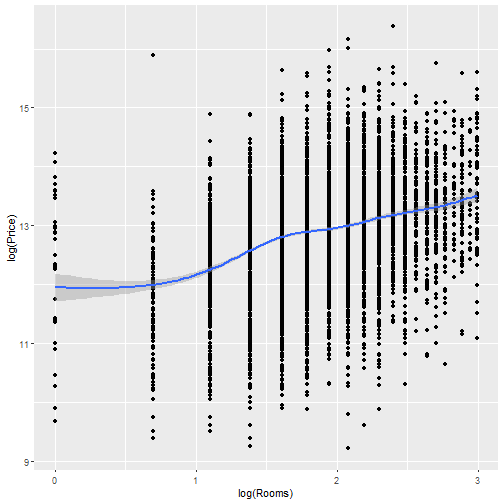
\includegraphics{Machine_Learning_Algorithms_Documentation_files/figure-latex/unnamed-chunk-68-1.pdf}
\includegraphics{Machine_Learning_Algorithms_Documentation_files/figure-latex/unnamed-chunk-68-2.pdf}

\begin{Shaded}
\begin{Highlighting}[]
\KeywordTok{write.table}\NormalTok{(res}\OperatorTok{$}\NormalTok{adj.values,}\StringTok{"out_abc.csv"}\NormalTok{, }\DataTypeTok{sep=}\StringTok{","}\NormalTok{, }\DataTypeTok{row.name=}\OtherTok{FALSE}\NormalTok{)}
\end{Highlighting}
\end{Shaded}

\end{document}
